\documentclass[10pt, a4paper, twocolumn, draft]{article}

\usepackage{stage}

\bibliography{biblio}

% Set stuff for title
\title{Shape-Adaptive Kernel Density Estimation}
\author{L.E.N. Baakman}

\begin{document}

\twocolumn[
  \begin{@twocolumnfalse}
    \maketitle
		\begin{abstract}
			%!TEX root = paper.tex
% Introduction
\noindent In numerous fields kernel density estimation is a popular method to approximate probability densities.
% Method
Generally these methods use symmetric kernels, even though the data of which the density is estimated are not necessarily spread equally in all dimensions. To account for this asymmetric distribution of data we propose the use of shape adaptive kernels: kernels whose shape changes to fit the spread of the data in the local neighborhood.
% Experiment
We compare the performance of the shape adaptive kernels with that of an estimator that uses a symmetric kernel on simulated data sets with known density fields.
% Results
No significant differences in performance between the symmetric and the shape-adaptive estimator were found, although the former outperformed the latter on points near the boundary of the data sets.  \todo[inline]{Say something about high-anisotropy}
% Conclusion
In conclusion shape-adaptive kernels are a promising idea that warrants further research.

		\end{abstract}
		\vspace{2em}
  \end{@twocolumnfalse}
]

\section{Introduction}
\label{s:introduction}
%!TEX root = paper.tex
Density estimation tries to find the density \varDensityFunction{\varPattern} in \varDim-dimensional Euclidean space underlying \varNumPatterns points $\varPattern[1] \dotsc \varPattern[\varNumPatterns]$, that have been selected independently from \varDensityFunction{\varPattern}. One often used method to solve this problem is the Parzen approach \cite{parzen1962estimation}, which gives the following estimate of the density function:
% Parzen
%
\begin{equation}\label{eq:1:parzen}
	\varEstimatedDensityFunction{\varPattern} = \frac{1}{\varNumPatterns}\sum_{j = 1}^{\varNumPatterns} \frac{1}{\varBandwidth^\varDim}\varKernel{\frac{\varPattern - \varPattern[j]}{\varBandwidth}}.
\end{equation}
%
Thus the estimated density is the mean of bumps placed at each observation. The shape of these bumps is determined by the shape of the kernel function \varKernel{\cdot}, their width is controlled by the bandwidth \varBandwidth \cite{silverman1986density}. The Parzen approach requires that $\varKernel{\varPattern} \geq 0$, with
% 
\begin{equation}\label{eq:1:kernelRequirement}
	\int \varKernel{\varPattern} = 1,
\end{equation}
it is often the case that the kernel statisfies some additional conditions. 

% Breiman, Meisel, Purcell
One downside of the Parzen method is that it cannot respond appropriately to variations in the magnitude of the density function, \ie the peakedness of the kernel is not data-responsive. Consequently in regions of low \varDensityFunction{\varPattern} that contain only one sample point, the estimate will have a peak at $\varPattern$ and be too low over the rest of the region. In areas where the density is high, the sample points are more densely packed together, and the Parzen estimate will tend to spread out the high density region \cite{breiman1977variable}. \citeauthor{breiman1977variable} introduced an variant of the Parzen estimator which makes the sharpness of the kernel responsive to the local data: 
%§
\begin{equation}\label{eq:1:BML}
 	\varEstimatedDensityFunction{\varPattern} = \frac{1}{\varNumPatterns} \sum_{j = 1}^{\varNumPatterns} (\varBMLconstant \varKNNDistance{j}{k})^{-\varDim} \varKernel[\varGaussian]{\frac{\varPattern - \varPattern[j]}{\varBMLconstant \varKNNDistance{j}{k}}},
\end{equation} 
%
where \varKernel[\varGaussian]{\cdot} represents a Gausian kernel, \varBMLconstant is a multiplicative constant and \varKNNDistance{j}{\KNNK} the distance between \varPattern[j] and the \KNNK nearest neighbour of \varPattern[j]. Comparing \cref{eq:1:parzen} with \eqref{eq:1:BML} we find that the bandwidth \varBandwidth, has been replaced with $\varBMLconstant \varKNNDistance{j}{\KNNK}$.  In low density regions \varKNNDistance{j}{\KNNK} will be large, and the kernel will be spread out, in high density regions the converse occurs. \citeauthor{breiman1977variable} use a minimization algorithm on a goodness of fit statistic to find suitable values for \KNNK and \varBMLconstant.

% % Ferdosi
One disadvantage of the Breiman estimator is that it is computationally expensive, both due to its minimization procedure and the infinite support kernel. \citeauthor{wilkinson1995dataplot} proposed the modified Breiman estimator:
%
	\begin{equation}\label{eq:1:bme}
		\varEstimatedDensityFunction{\varPattern} = \frac{1}{\varNumPatterns} \sum_{j = 1}^{\varNumPatterns} \left(\varBandwidth \varLocalBandwidth{j} \right)^{- \varDim} \varKernel[\varEpan]{\frac{\varPattern - \varPattern[j]}{\varBandwidth \varLocalBandwidth{j}}}.
	\end{equation}
%
This estimator differs on two points from the Breiman estimator. Firstly contrary to \citeauthor{breiman1977variable} who use a Gaussian kernel, \citeauthor{ferdosi2011comparison} use an Epanechnikov kernel \cite{epanechnikov1969non}. Secondly they replaced the expensive minimization procudure with a pilot density estimate:
% 
	\begin{equation}\label{eq:1:mbePilot}
		\varPilotDensityFunction{\varPattern} = \frac{1}{\varNumPatterns} \sum_{j = 1}^{\varNumPatterns} \varBandwidth^{- \varDim} \varKernel{\frac{\varPattern - \varPattern[j]}{\varBandwidth}}.
	\end{equation}
%
By computing the pilot density first on grid points and using multi-linear interpolation to determine the pilot density for each point the computational complexity is further decreased. 
Based on these pilot densities the local bandwidths are computed:
	\begin{equation}\label{eq:1:mbeLocalBandwidth}
		\varLocalBandwidth{i} = \left( \frac{\varPilotDensityFunction{\varPattern[i]}}{\varGeometricMean}
		\right)^{-\varMBESensitivityParam}.
	\end{equation}
Here \varGeometricMean is the geometric mean of the pilot densities and \varMBESensitivityParam is the sensitivity parameter. 

Although the widths of the kernels used in both the Breiman estimator and the modified Breiman estimator respond to the data, the shapes of the kernels are dependent of the kernel not the data. To further increase the response of the estimator to the data we propose shape-adaptive kernels, kernels of which both the width and the shape are steered by the data. 

A disadvantage of these shape-adaptive kernels is that in regions where the density of sample points is low there are not enough data points to compute the shape of the kernel reliably. Consequently we propose to let the amount in which the shape of the kernel is influenced by the local data depend on their density. 

This paper is organized as follows. \Cref{s:method} discusses the proposed shape-adaptive kernels and somee implementation details. \todo{Aanvullen}

\begin{table*}[th!]
	\centering
	%!TEX root = ../../paper.tex
\small
\sisetup{
	table-format=5.0,
	scientific-notation=false,
	round-mode=places,
	round-precision=1,
	table-number-alignment=center
}
\renewcommand{\arraystretch}{1.2}
\begin{tabular}{@{}cclSl@{}}
\toprule
				&~						& Component					& {Samples} 	& Distribution\\
\midrule
% Ferdosi 1
\ferdosiOne 	&\legendComponentOne	& Trivariate Gaussian 		& 40000		& $\gaussDist{[50, 50, 50]}{\diag(11)}$\\
~ 				&\legendComponentNoise	& Uniform random background	& 20000		& $\uniformDist{[0, 0, 0]}{[100, 100, 100]}$\\
% Baakman 1
\hline
\baakmanOne		&\legendComponentOne	& Trivariate Gaussian 		& 40000		& $\gaussDist{[50, 50, 50]}{\diag([11^2, \sqrt{11}, \sqrt{11}])}$\\
~ 				&\legendComponentNoise	& Uniform random background	& 20000		& $\uniformDist{[0, 0, 0]}{[100, 100, 100]}$\\
% Baakman 4
\hline
\baakmanFour	&\legendComponentOne	& Trivariate Gaussian 		& 40000		& $\gaussDist{[50, 50, 50]}{\diag([11^2, 2 * \sqrt{11}, \rfrac{1}{2} \sqrt{11}])}$\\
~ 				&\legendComponentNoise	& Uniform random background	& 20000		& $\uniformDist{[0, 0, 0]}{[100, 100, 100]}$\\
% Baakman 5
\hline
\baakmanFive	&\legendComponentOne	& Trivariate Gaussian 		& 40000		& $\gaussDist{[50, 50, 50]}{\diag([11^2, 11, 1])}$\\
~ 				&\legendComponentNoise	& Uniform random background	& 20000		& $\uniformDist{[0, 0, 0]}{[100, 100, 100]}$\\
\bottomrule
\end{tabular}
	\caption{The data sets containing a single Gaussian distribution embedded in uniform noise. The column `Number' indicates for each component the number of patterns sampled from it. \gaussDist{\varMean}{\varCovarianceMatrix} denotes a Gaussian distribution with mean \varMean and covariance matrix \varCovarianceMatrix. A diagonal matrix with the values $x_1,\, \dotsc,\, x_\varDim$ on the diagonal is represented as $\diag([x_1,\,\dotsc,\,x_\varDim]])$, a scalar matrix with $x$ on the diagonal is shown as $\diag(x)$. \uniformDist{a}{b} denotes a uniform distribution with its minimum and maximum set to $a$ and $b$, respectively. The second column presents the symbol used to represent this component in plots throughout the paper.} 	
	\label{tab:experiment:singlesphere:sets}
\end{table*}

\section{Method}
\label{s:method}
%!TEX root = paper.tex

%General Idea
	We use our shape adaptive kernels in combination with the Modified Breiman Estimator introduced by \textcite{wilkinson1995dataplot}. The grid used for the pilot densities is 
	%Pilot Densities
	The grid that the pilot densities are computed on \todo{Iets over hoe het grid bepaald wordt, of de standaard grootte van het grid.} 
	%General bandwidth
	We choose to use the method proposed by \textcite{ferdosi2011comparison} for computing the general bandwidth because of its lower complexity, compared to the method used by \textcite{wilkinson1995dataplot}. 
	%Local bandwidths
	We have empirically determined \todo{hoe hebben we dat vastgesteld} that using \varMBESensitivityParam = \todo{Een of andere waarde} works best in our case. 
	%Final densities
	The final densities are estimated according to \cref{eq:1:adaptiveKernelEstimateWithLocalBandwidths} with a reshaped and scaled Epanechnikov kernel. The Epanechnikov kernel reshaped with the matrix \varCovarianceMatrix is defined as:
	\begin{equation}\label{eq:1:epanechnikovKernelWithCovarianceMatrix}
		\varKernel[\varEpan]{\varPattern} = 
		\begin{cases}
			\frac{\varDim + 2}{2\varUnitSphere{\varDim}} \left( 1 - \varPattern \varCovarianceMatrix \varPattern \right) & \text{if } \varPattern \cdot \varPattern < 1\\
			0 & \text{otherwise.}
		\end{cases}
	\end{equation}
	As stated before the matrix \varCovarianceMatrix is determined based on the neighborhood of the pattern, \varPattern, whose density we are estimating. 

	We determine the neighbors of \varPattern with the \KNNK nearest neighbors algorithm (\KNN) with Euclidean distance. This approach is used rather than a fixed-radius neighborhood to ensure that independent of the sparsity of the data the kernel shape is always based on a reasonable number of data points. Furthermore using \KNN allows us to choose $\KNNK > \varDim$, which makes it extremely improbable that the covariance matrix of the neighborhood is singular. We follow \citeauthor{silverman1986density}'s \cite{silverman1986density} recommendation of choosing $k = \sqrt{\varNumPatterns}$. To ensure that even in high-dimensional data sets $\KNNK > \varDim$ we use
	\begin{equation*}
	\KNNK = \max\left(\sqrt{\varNumPatterns},\, \varDim + 1\right).	
	\end{equation*}
	Let \varNeighborhood{\varPattern} denote the union of \varPattern and its neighborhood, the basic shape of the kernel used for \varPattern is then given by \varCovarianceFunction{\varNeighborhood{\varPattern}}.

	To allow the density estimation of each pattern to be influenced by an equal area, before the application of the smoothing factor $\varLocalBandwidth{i}$, the basic shapes of the kernels need to be scaled. To that end we use the eigenellipse, the ellipse defined by the eigenvectors and eigenvalues of \varCovarianceFunction{\varNeighborhood{\varPattern}}. We scale the covariance matrix with the factor \varScalingFactor, defined as:
	\begin{equation}
		\varScalingFactor = \frac{\varBandwidth^2}{\varGeometricMeanFunction{\sqrt{\lambda_1}, \dotsc, \sqrt{\lambda_\varDim}}},
	\end{equation}
	where $\lambda_j$ denotes the $j$th eigenvalue of the $j$th eigenvector of \varCovarianceMatrix. The scaling factor \varScalingFactor ensures that the shape-adapted covariance matrix has the same scale as the covariance matrix that is implicitly used in the Modified Breiman Estimator with a Gaussian kernel.

\section{Experiments}
\label{s:experiment}
%!TEX root = ../paper.tex
This section discusses the previously presented results. We first consider the lack of difference in performance between the two estimators. The section after that is concerned with the anisotropy of the kernels used by the shape-adaptive estimator. Finally we offer some directions research into solving the identified issues might take.

\subsection{Performance}
\label{s:discussion:performance}
%!TEX root = ../paper.tex

% Hardly any difference between estimators
One of the most striking observations from \cref{s:results} is that the difference in performance between the two estimators is minimal. 
	
	% Study differences further mbe vs sambe plot
		% Single Sphere Sets
		Plotting the densities estimated by \sambe as a function of those estimated by \mbe shows no interesting differences between the two estimators for data set \ferdosiOne through \baakmanFive. 
		% Multi Sphere Sets
		However for data set \ferdosiTwo through \baakmanThree these plots reveal some differences between the estimators. As can be seen in \cref{fig:discussion:performance:two:mbevssambe}, using shape-adaptive kernels results in estimated densities that are generally higher than those estimated with a fixed-shape kernel for data set \ferdosiTwo and \baakmanTwo. Reviewing the raw data shows that \sambe underestimates densities less than \mbe on points near the mean of `Trivariate Gaussian 1'. The kernels in this neighborhood are all slightly anisotropic, which has allowed the shape-adaptive estimator to use more data points, to better approximate the local densities. Thus showing that estimating densities with shape-adaptive kernels can be advantageous.
		%
		\begin{figure}
			\centering
			\begin{subfigure}{0.3\textwidth}
				\centering
				\includegraphics[keepaspectratio=true, width=\textwidth, height=0.23\textheight]{discussion/img/ferdosi_2_60000_mbe_sambe.png}
				\caption{Data set \ferdosiTwo}
				\label{fig:discussion:performance:mbevssambe:ferdosi2}
			\end{subfigure}
			\subfigvspace
			\begin{subfigure}{0.3\textwidth}
				\centering
				\includegraphics[keepaspectratio=true, width=\textwidth, height=0.23\textheight]{discussion/img/baakman_2_60000_mbe_sambe.png}
				\caption{Data set \baakmanTwo}
				\label{fig:discussion:performance:mbevssambe:baakman2}
			\end{subfigure}	
			\caption{Plots of the densities estimated by \sambe as a function of those estimated by \mbe for data set %
				\subref{fig:discussion:performance:mbevssambe:ferdosi2} % 
				\ferdosiTwo and %
				\subref{fig:discussion:performance:mbevssambe:baakman2} %
				\baakmanTwo.
			}
			\label{fig:discussion:performance:two:mbevssambe}
		\end{figure}
		
		% Ferdosi 3 / Baakman 3
		\Cref{fig:discussion:performance:four:mbevssambe} shows the opposite effect; the densities estimated by \sambe for data set \ferdosiThree and \baakmanThree are generally lower than those estimated by \mbe. Reviewing the raw data shows that the points where the differences in estimated densities between the two estimators are largest lie near the mean of the `Trivariate Gaussian 3' in both data set \ferdosiThree and \baakmanThree. The number of points used in the density estimate by \sambe is consistently lower than the number of points used by the fixed-shape estimator. Given the relatively high anisotropy of the kernels in that area we expect that this is due to the kernels reflecting fine local structures, instead of the global neighborhood. 
		%	
		\begin{figure}
			\centering
			\begin{subfigure}{0.3\textwidth}
				\centering
				\includegraphics[keepaspectratio=true, width=\textwidth, height=0.23\textheight]{discussion/img/ferdosi_3_120000_mbe_sambe.png}
				\caption{Data set \ferdosiThree}
				\label{fig:discussion:performance:mbevssambe:ferdosi3}
			\end{subfigure}
			\subfigvspace
			\begin{subfigure}{0.3\textwidth}
				\centering
				\includegraphics[keepaspectratio=true, width=\textwidth, height=0.23\textheight]{discussion/img/baakman_3_120000_mbe_sambe.png}
				\caption{Data set \baakmanThree}
				\label{fig:discussion:performance:mbevssambe:baakman3}
			\end{subfigure}	
			\caption{Plots of the density estimated by \sambe as a function of those estimated by \mbe for data set %
				\subref{fig:discussion:performance:mbevssambe:ferdosi3} % 
				\ferdosiThree and %
				\subref{fig:discussion:performance:mbevssambe:baakman3} %
				\baakmanThree.
			}
			\label{fig:discussion:performance:four:mbevssambe}
		\end{figure}

	% Where are the differences largest -> plots
	% Single Sphere
		\begin{figure}
			\centering
			\begin{subfigure}{0.23\textwidth}
				\centering
				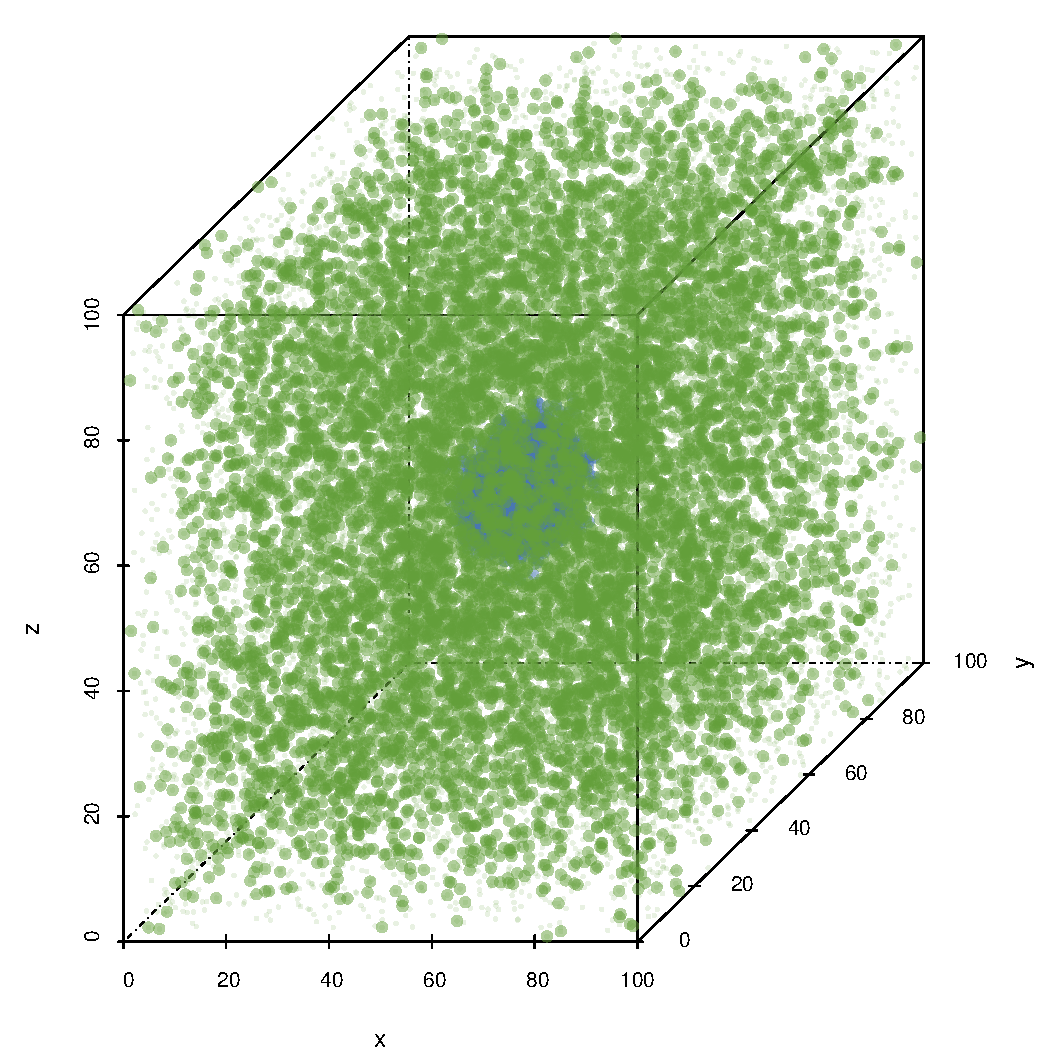
\includegraphics[keepaspectratio=true, width=\textwidth, height=0.23\textheight]{discussion/img/ferdosi_1_abs_error_mbeSmallerThansambe}
				\caption{Data set \ferdosiOne}
				\label{fig:discussion:performance:mbeLowerError:ferdosi1}
			\end{subfigure}
			\begin{subfigure}{0.23\textwidth}
				\centering
				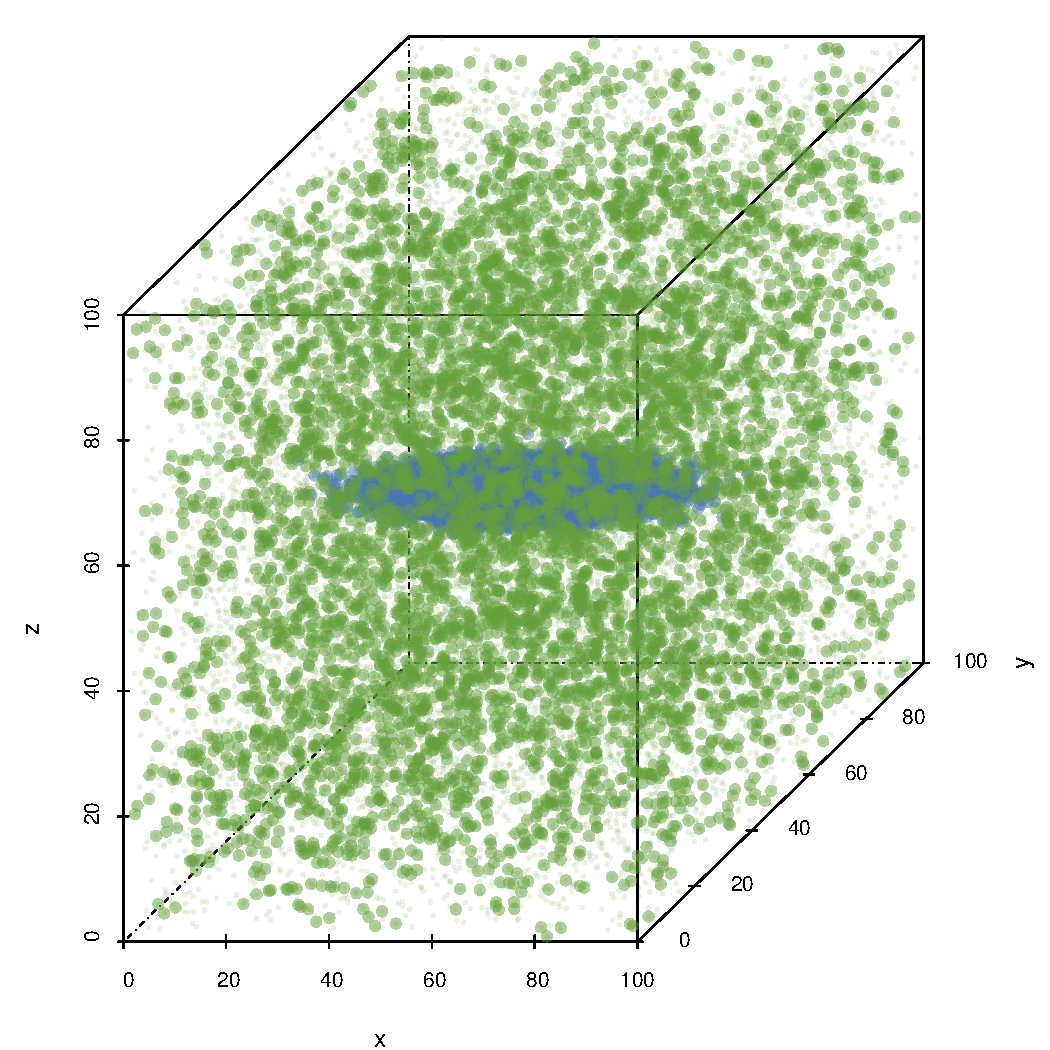
\includegraphics[keepaspectratio=true, width=\textwidth, height=0.23\textheight]{discussion/img/baakman_1_abs_error_mbeSmallerThansambe}
				\caption{Data set \baakmanOne}
				\label{fig:discussion:performance:mbeLowerError:baakman1}
			\end{subfigure}	
			\subfigvspace
			\begin{subfigure}{0.23\textwidth}
				\centering
				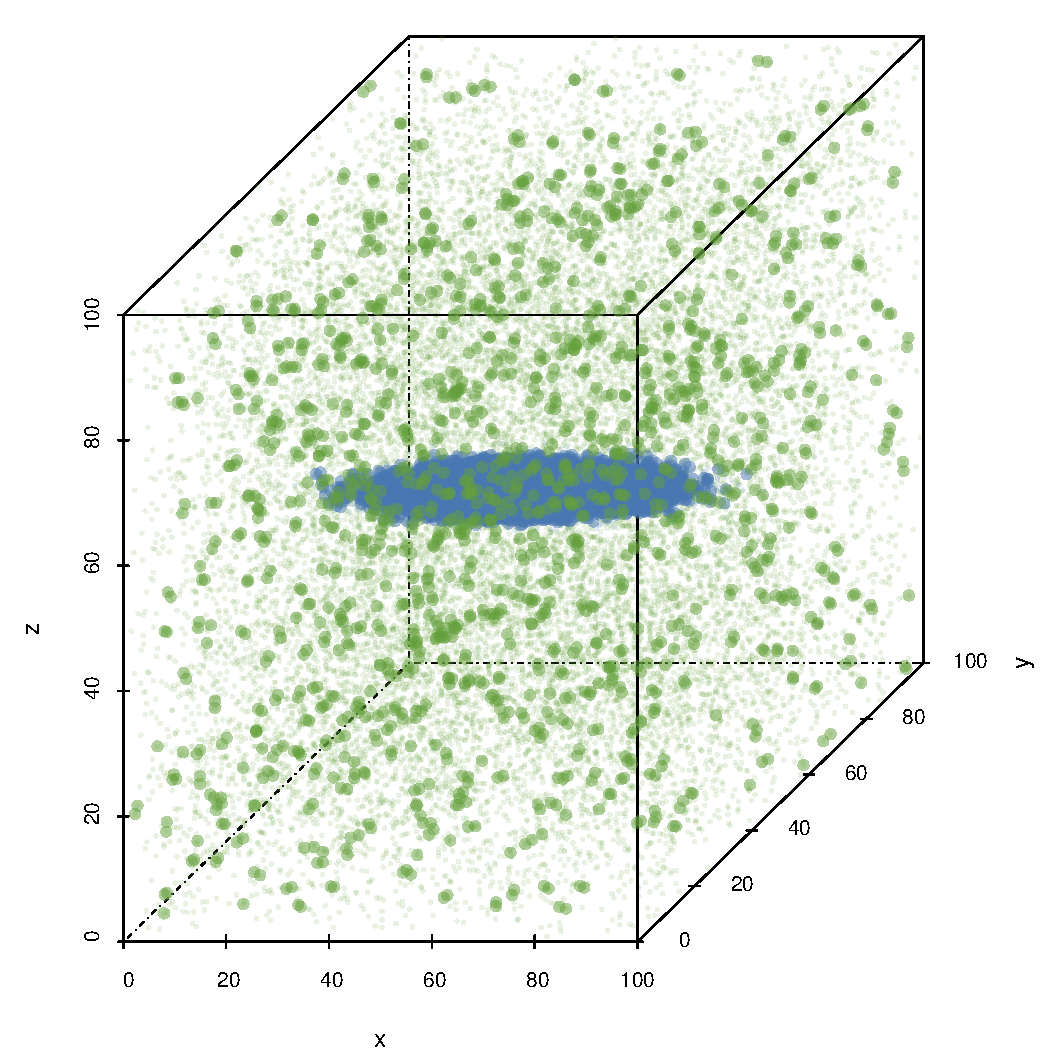
\includegraphics[keepaspectratio=true, width=\textwidth, height=0.23\textheight]{discussion/img/baakman_4_abs_error_mbeSmallerThansambe}
				\caption{Data set \baakmanFour}
				\label{fig:discussion:performance:mbeLowerError:baakman4}
			\end{subfigure}		
			\begin{subfigure}{0.23\textwidth}
				\centering
				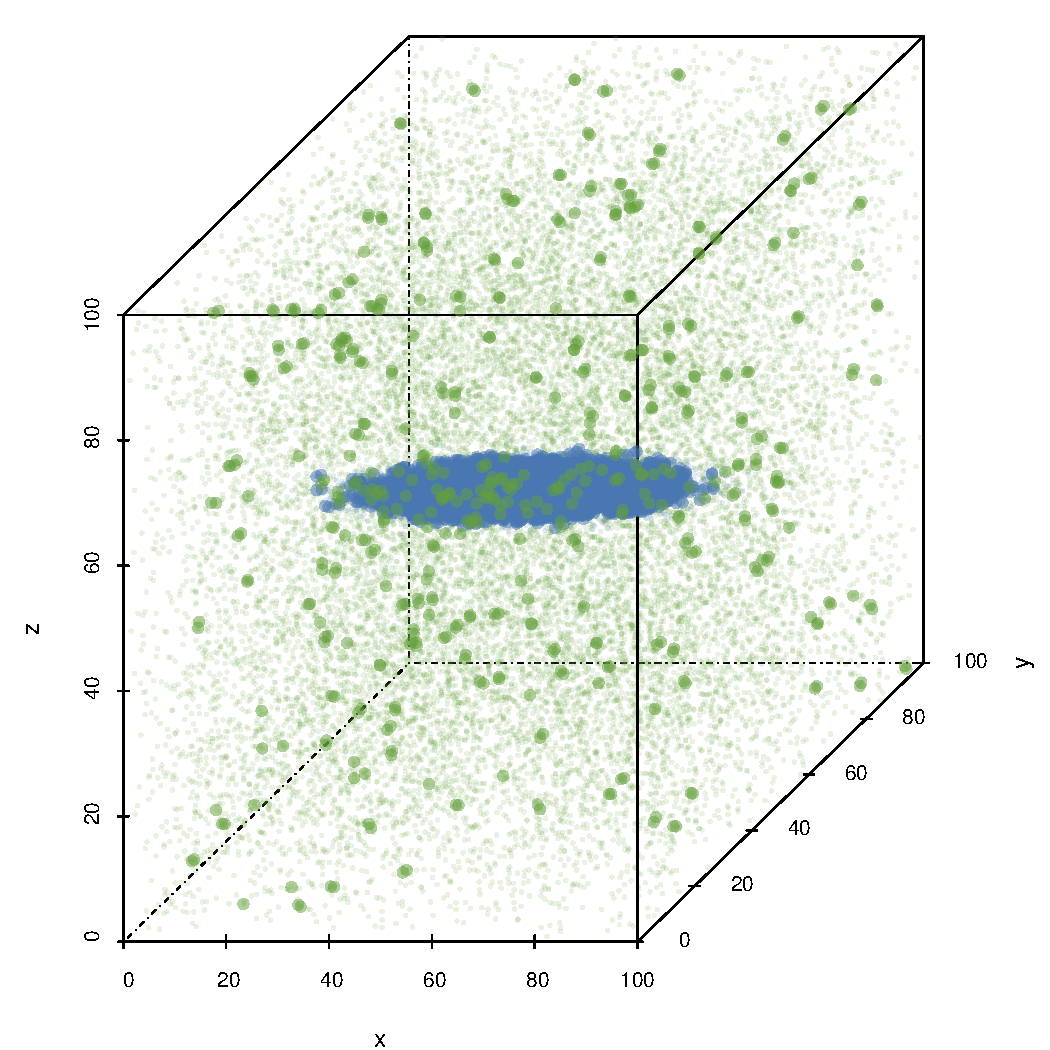
\includegraphics[keepaspectratio=true, width=\textwidth, height=0.23\textheight]{discussion/img/baakman_5_abs_error_mbeSmallerThansambe}
				\caption{Data set \baakmanFive}
				\label{fig:discussion:performance:mbeLowerError:baakman5}
			\end{subfigure}			
			\caption{Low opacity scatter plot of data set %
				\subref{fig:discussion:performance:mbeLowerError:ferdosi1} \ferdosiOne, %
				\subref{fig:discussion:performance:mbeLowerError:baakman1} \baakmanOne, %
				\subref{fig:discussion:performance:mbeLowerError:baakman4} \baakmanFour, and %
				\subref{fig:discussion:performance:mbeLowerError:baakman5} \baakmanFive, %
				with an overlay of larger, colored points where the absolute error of \sambe is larger than the absolute error of \mbe.}
			\label{fig:discussion:performance:singleSphere:mbeLowerError}
		\end{figure}
		%	
		The plots in \cref{fig:discussion:performance:singleSphere:mbeLowerError} emphasize the points in data set \ferdosiOne and \baakmanOne where the absolute error of \mbe is smaller than that of \sambe. These plots show that the shape-adaptive kernels outperform symmetric kernels near the borders of the data sets.
			% Why the boundary effect
			We expect that this boundary effect is due to the strong anisotropy of the local neighborhood of the points near the limits of the data sets. Consequently the domain of the shape-adaptive kernels extends less outside of the boundaries of the data set than the domains of the symmetric kernels. This results in less underestimation of densities near the boundary of the data set, if shape-adaptive kernels are used.
			% Why is it stonger of the Gaussian is more anisotropic
			Furthermore the strength of the boundary effect seems to increase as the Gaussian component of the data set is more anisotropic. However the seemingly better performance of \sambe is due to an increase in the number of points where the density estimated by \sambe equals the density estimated by \mbe. In data set \ferdosiOne the two estimators give a different result on all points. In data set \baakmanOne the estimators agree on the density of \percentage{1.327294605254362e+01} of the points, this increases to \percentage{3.535329901731399e+01} in data set \baakmanFive.
			%SAMBE == MBE
			%Ferdosi 1 (0.000000000000000e+00 percent)
			%Baakman 1 (1.327294605254362e+01 percent)
			%Baakman 4 (2.989838892974129e+01 percent)
			%Baakman 5 (3.535329901731399e+01 percent)
			As the Gaussian component becomes more anisotropic the number of points whose local neighborhood consists only of uniform noise increases. On average the covariance matrix of neighborhoods that contain primarily points sampled from the noise component should be scalar. Consequently as the anisotropy of the Gaussian component increases more shape-adaptive kernels take on a shape that is near-symmetric. This results in points were both estimators give the same approximated density. 
	
	% Multi Sphere
		\begin{figure}
			\centering
			\begin{subfigure}{0.23\textwidth}
				\centering
				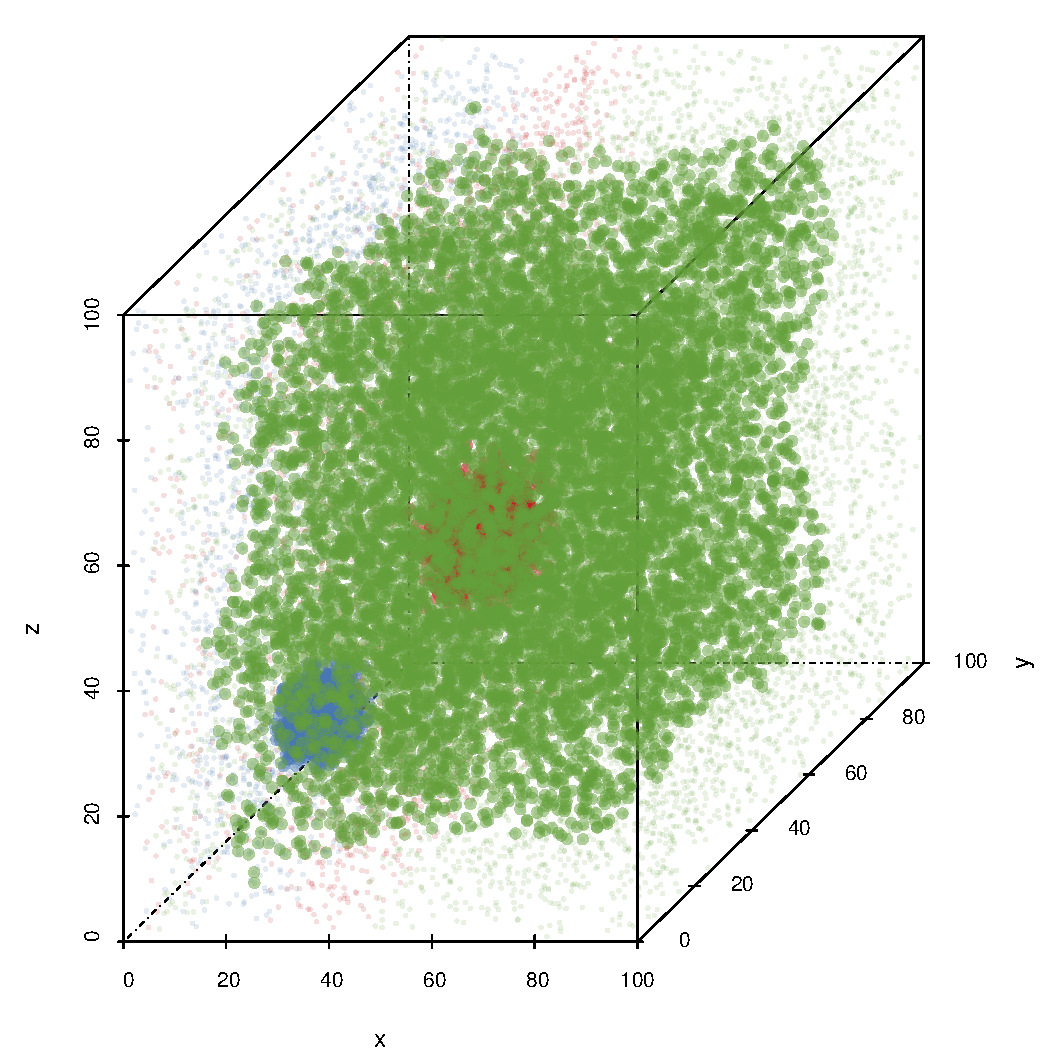
\includegraphics[keepaspectratio=true, width=\textwidth, height=0.23\textheight]{discussion/img/ferdosi_2_abs_error_mbeSmallerThansambe}
				\caption{Data set \ferdosiTwo}
				\label{fig:discussion:performance:mbeLowerError:ferdosi2}
			\end{subfigure}
			\begin{subfigure}{0.23\textwidth}
				\centering
				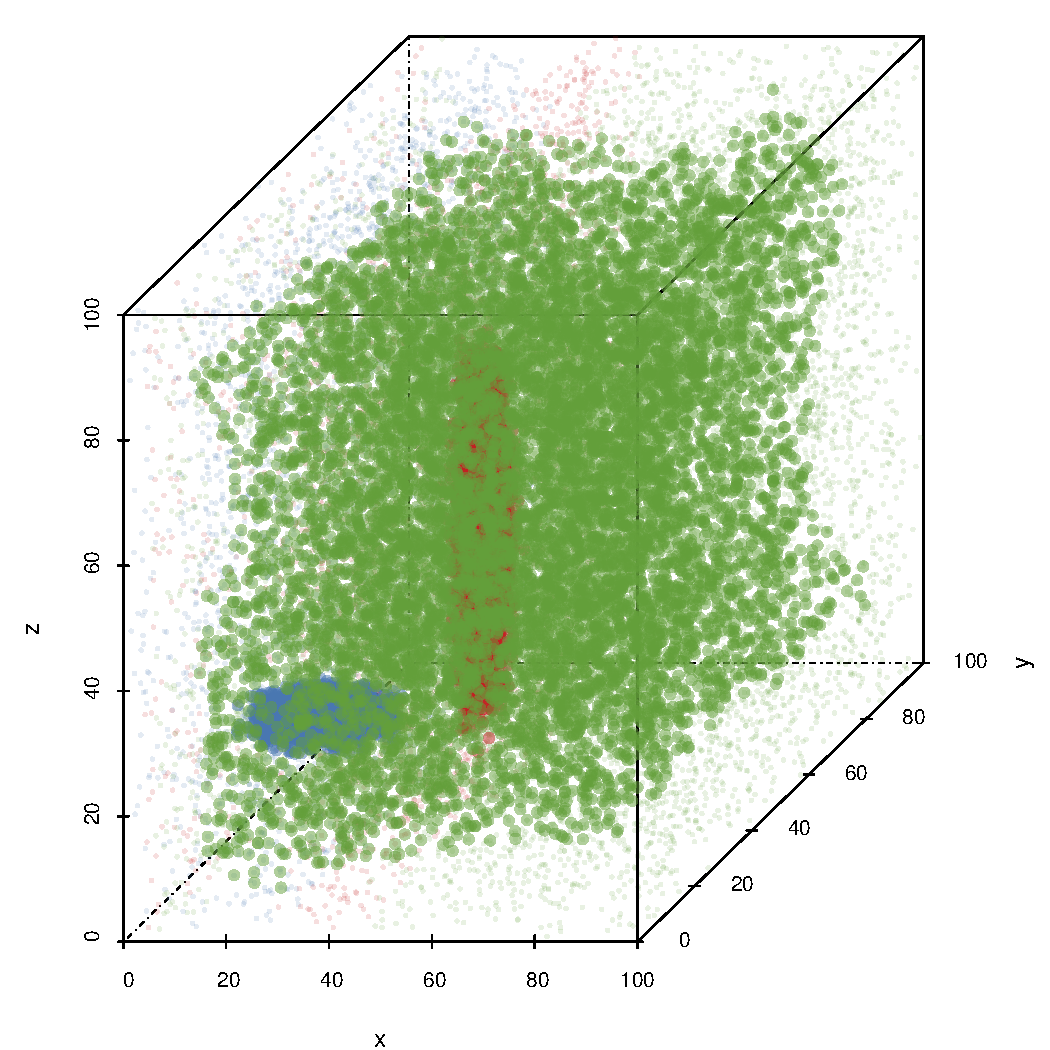
\includegraphics[keepaspectratio=true, width=\textwidth, height=0.23\textheight]{discussion/img/baakman_2_abs_error_mbeSmallerThansambe}
				\caption{Data set \baakmanTwo}
				\label{fig:discussion:performance:mbeLowerError:baakman2}
			\end{subfigure}	
			\subfigvspace
			\begin{subfigure}{0.23\textwidth}
				\centering
				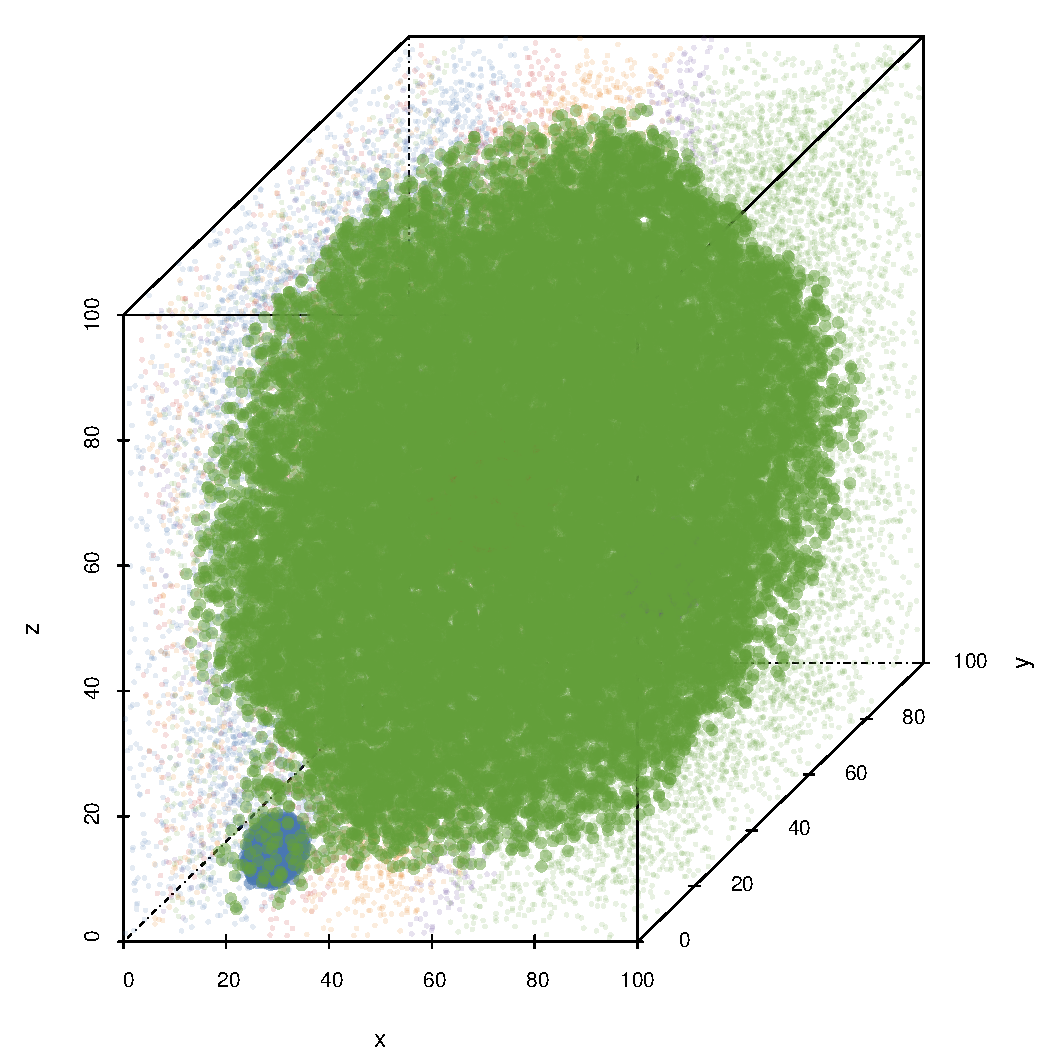
\includegraphics[keepaspectratio=true, width=\textwidth, height=0.23\textheight]{discussion/img/ferdosi_3_abs_error_mbeSmallerThansambe}
				\caption{Data set \ferdosiThree}
				\label{fig:discussion:performance:mbeLowerError:ferdosi3}
			\end{subfigure}
			\begin{subfigure}{0.23\textwidth}
				\centering
				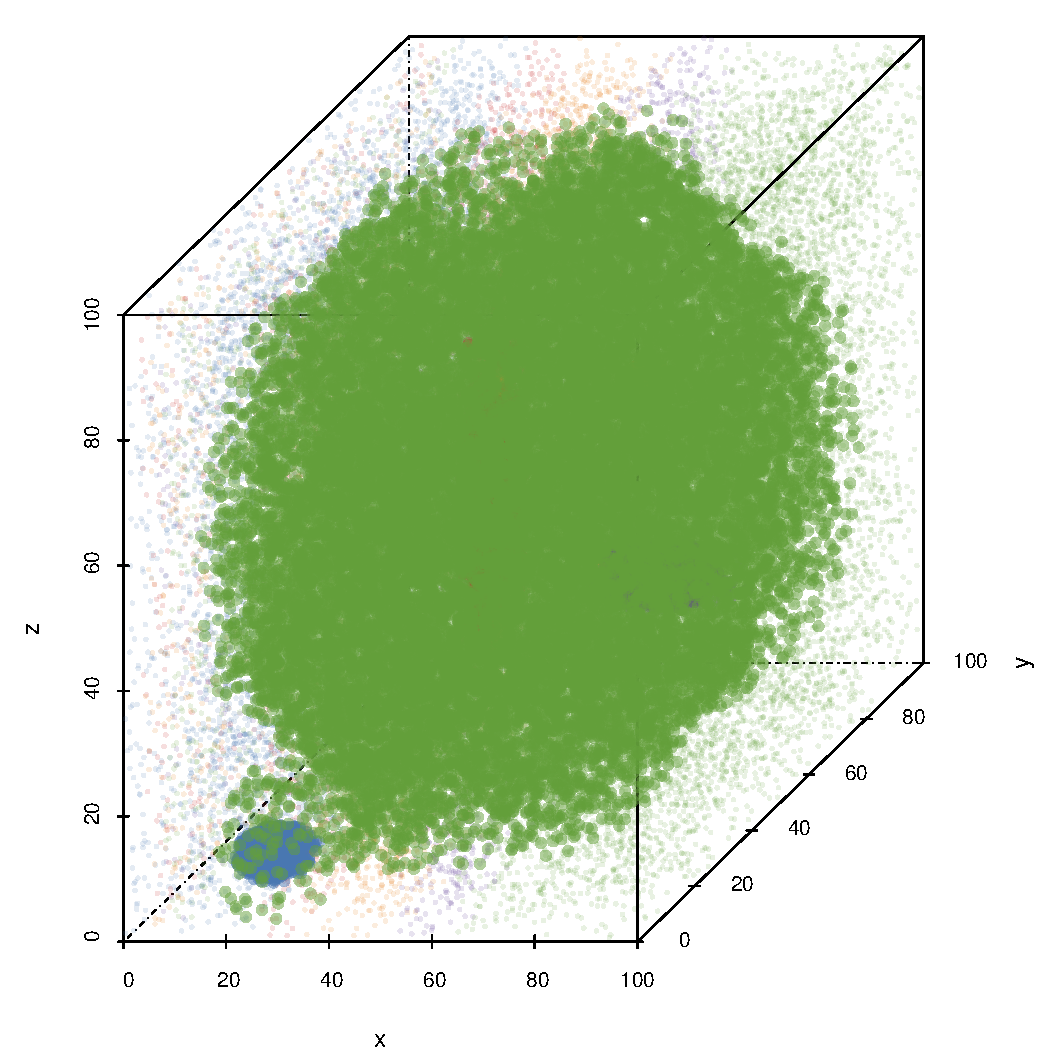
\includegraphics[keepaspectratio=true, width=\textwidth, height=0.23\textheight]{discussion/img/baakman_3_abs_error_mbeSmallerThansambe}
				\caption{Data set \baakmanThree}
				\label{fig:discussion:performance:mbeLowerError:baakman3}
			\end{subfigure}			
			\caption{Low opacity scatter plot of data set %
				\subref{fig:discussion:performance:mbeLowerError:ferdosi2} \ferdosiTwo, %
				\subref{fig:discussion:performance:mbeLowerError:baakman2} \baakmanTwo, %
				\subref{fig:discussion:performance:mbeLowerError:ferdosi3} \ferdosiThree, and %
				\subref{fig:discussion:performance:mbeLowerError:baakman3} \baakmanThree %
				with an overlay of high opacity, larger points where the absolute error of \mbe is smaller than that of \sambe.}
			\label{fig:discussion:performance:multisphere:mbeLowerError}
		\end{figure}	
		The points where using fixed-shape kernels results in a smaller error in data sets \ferdosiTwo through \baakmanThree are emphasized in
		\cref{fig:discussion:performance:multisphere:mbeLowerError}. We contribute the boundary effect in these data sets to the same cause as the boundary effect in the data sets with a single Gaussian component. Interestingly the points in data set \ferdosiThree and \baakmanThree where the absolute error of \mbe is lower, approximate a sphere, contrary to the cube they define for data set \ferdosiTwo and \baakmanTwo. It is our expectation that this is caused by the smaller distance between the means of the Gaussian components and the range of the uniform random background in \ferdosiThree and \baakmanThree.
			% Define Ferdosi 3 Noise
			To test this we define data set \ferdosiThreeNoise, which replaces the uniform random background of \ferdosiThree with $\uniformDist{[-20, -20, -20]}{[120, 120, 120]}$. We adjust the number of points sampled from this component to ensure that its density is equal to that of the noise component of \ferdosiThree.
			% Is there any effect on the MSE
			The overall \mse of both estimators is slightly smaller for data set \ferdosiThreeNoise than for \ferdosiThree, however the \mse of `Trivariate Gaussian 1' and 3 shows a small increase. 
			% Did the distance to the boundaries explain it?
			\Cref{fig:discussion:ferdosi3Noise:mbeLowerError} confirms that the spherical shape in \cref{fig:discussion:performance:mbeLowerError:ferdosi3,fig:discussion:performance:mbeLowerError:baakman3} is caused by the Gaussian near the boundary of the data set. As the shape defined by the emphasized points is now a cubical instead of spherical. 
			% The Plots of Ferdosi 3 Noise
			\begin{figure}
				\centering
				\begin{subfigure}{0.23\textwidth}
					\centering
					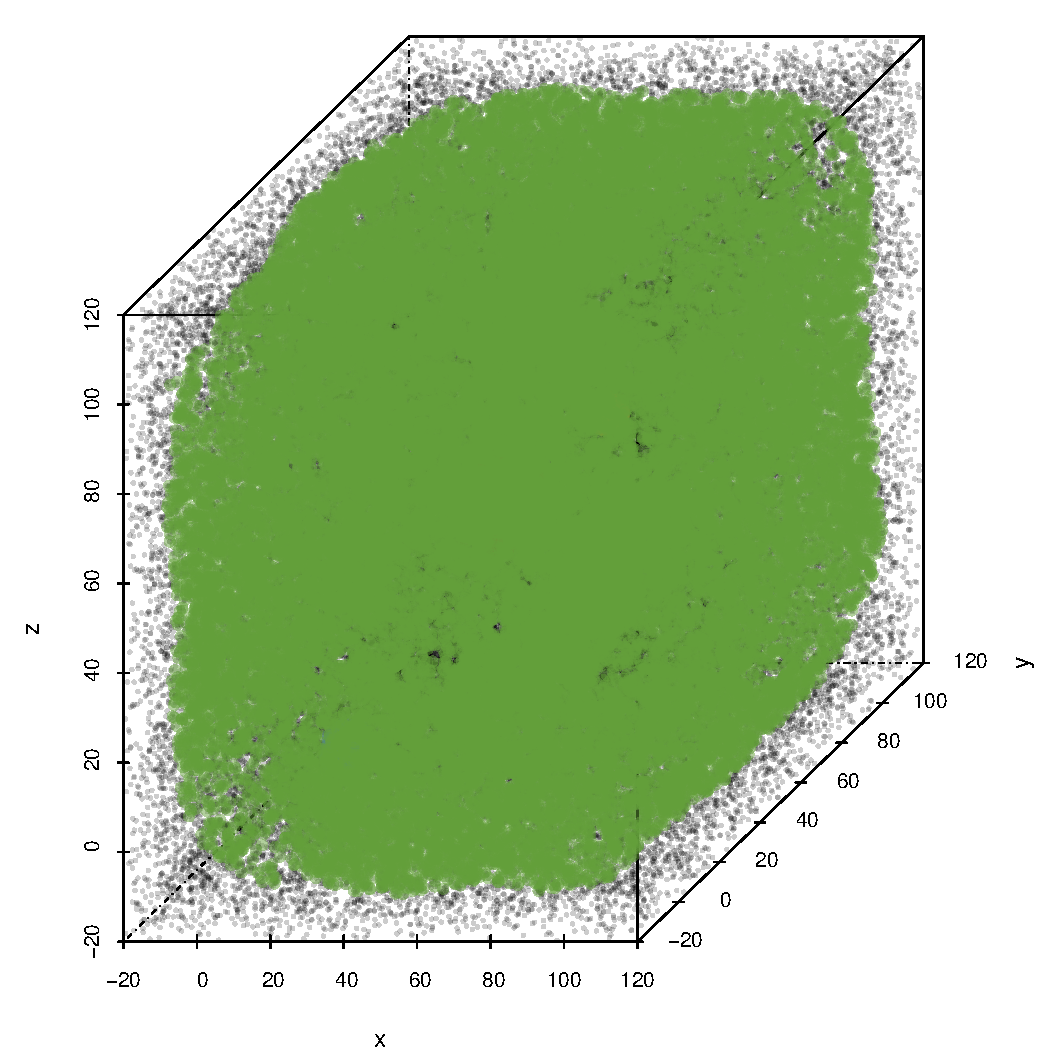
\includegraphics[keepaspectratio=true, width=\textwidth, height=0.23\textheight]{discussion/img/ferdosi_3_more_noise_abs_error_mbeSmallerThansambe.png}
					\caption{Absolute Error}
					\label{fig:discussion:ferdosi3Noise:mbeLowerError}
				\end{subfigure}		
				\begin{subfigure}{0.23\textwidth}
					\centering
					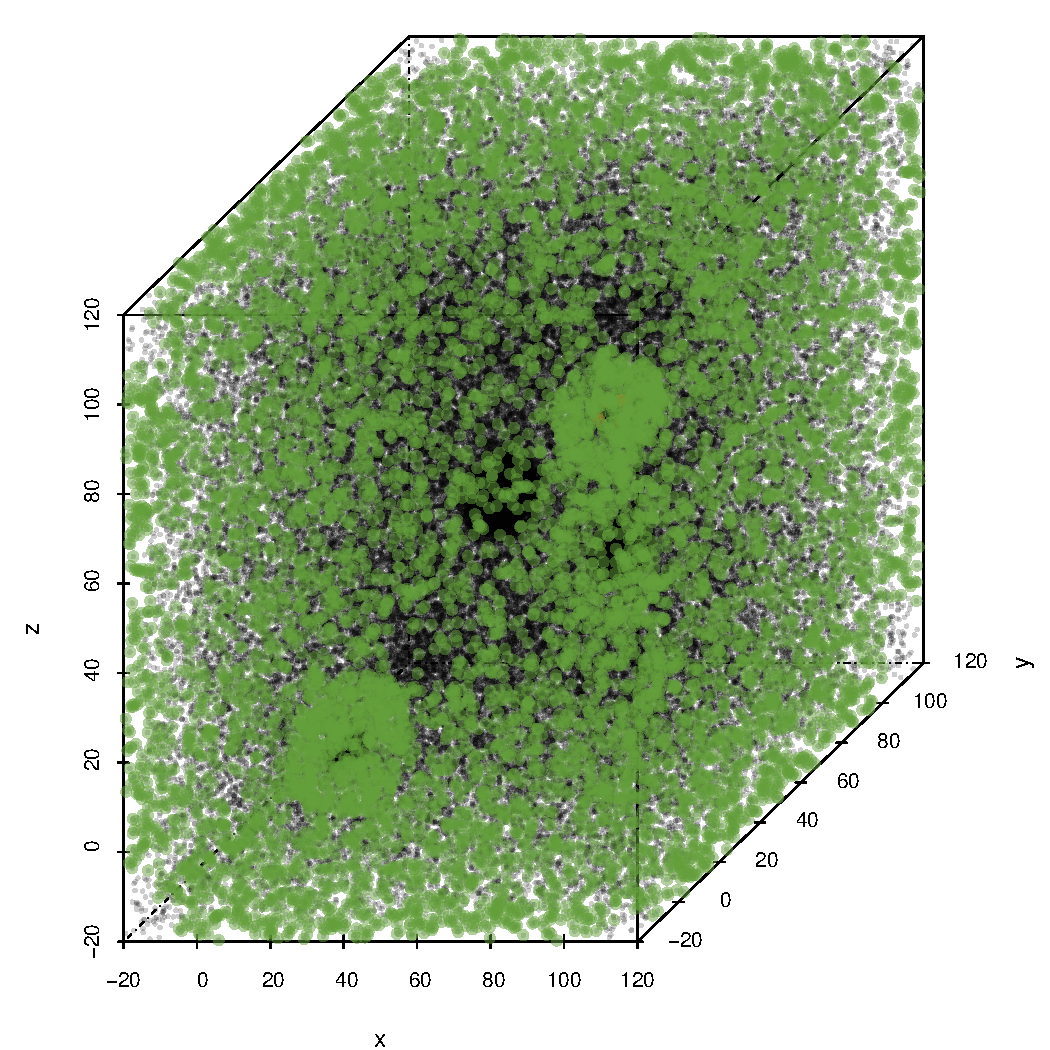
\includegraphics[keepaspectratio=true, width=\textwidth, height=0.23\textheight]{discussion/img/ferdosi_3_more_noise_anisotropy.png}
					\caption{Anisotropy}
					\label{fig:discussion:ferdosi3Noise:anisotropy}
				\end{subfigure}			
				\caption{Low opacity scatter plot of data set \ferdosiThreeNoise with %
					\subref{fig:discussion:ferdosi3Noise:mbeLowerError} points where the absolute error of \mbe is lower than that of \sambe and %
					\subref{fig:discussion:ferdosi3Noise:anisotropy} points sampled from the Gaussian components with kernels whose anisotropy falls in the \nth{95} percentile of the complete data set emphasized.}
				\label{fig:discussion:ferdosi3Noise}
			\end{figure}		

% Some conclusion
To conclude we have found that shape-adaptive kernels definitely improve performance in some cases, \ie near the boundary of the data sets and near the mean of some Gaussian components. Unfortunately in other cases the anisotropic kernels are detrimental. The difference in \mse between the two estimators shows that generally, using fixed-shape kernels is slightly advantageous. 

\subsection{Kernel Anisotropy}
\label{s:discussion:anisotropy}
%!TEX root = ../paper.tex

% Small differences in anisotropy  
	% Where are the differeneces largest -> plots
	% Refer to earlier solutions

% Highest anisotropy of noise component 
	% Kernel 'catches' spurious structures in noise -> increase K.

% 	  Denser component -> higher anisotropy of kernels
% AND Higher anistropy in component -> higer anisotropy in associated kernels
% AND Denser comonent -> lower MSE
	% Introduce the dataset A1 and A2, same anisotropy different density, what do we observe, what does it say about this correlation.

% Lack of difference in anisotropy between F3 and B3 in orange (‘Trivariate Gaussian 3’) component. 

We have found that near Gaussian components with a high volume eigensphere the kernels are too isotropic, whereas in the uniform random background fine structures are detected that result in too anisotropic kernels. Both of these problems might be solved by increasing the value of \KNNK. 
% Effect on noise:
We expect that increasing the size of the local neighborhood will decrease the number of detected fine structures. Which results in more isotropic kernels for points that lie in the uniform background.
% Effect on low density gaussians: 
Furthermore increasing the size of the local neighborhood might also allow the kernels to adapt their shape to nearby Gaussian components whose eigensphere has a high volume. Multiplying the \KNNK computed in \cref{eq:method:k} by ten, resulted in \sambe outperforming \mbe on dataset \baakmanFive. Furthermore the increased \KNNK also improved the performance on dataset \ferdosiThree, \baakmanThree and the datasets with a single Gaussian components. Whereas the performance of \sambe on dataset \ferdosiTwo and \baakmanTwo decreased. This suggest that blindly increasing the size of the local neighborhood will not consistently improve the performance of the estimator, but that same adaptive increase of \KNNK is required.

Another solution to the too anisotropic kernels in the noise might be to only use shape-adaptive kernels if the neighborhood is sufficiently anisotropic. One might even consider using a kernel-shape that is somewhere between the isotropic and the fully anisotropic kernel depending on the anisotropy of the local neighborhood. A difficulty with this approach is detecting the isotropy of the local neighborhood. As the obvious solution, the covariance matrix, has proven sensitive to fine structures within the noise. 

Finally the correlation between the performance of the estimators and the volume of the eigensphere of the Gaussian component suggests that the method used to compute the local bandwidths is far from ideal. 

\section{Results}
\label{s:results}
%!TEX root = ../paper.tex
This section discusses the previously presented results. We first consider the lack of difference in performance between the two estimators. The section after that is concerned with the anisotropy of the kernels used by the shape-adaptive estimator. Finally we offer some directions research into solving the identified issues might take.

\subsection{Performance}
\label{s:discussion:performance}
%!TEX root = ../paper.tex

% Hardly any difference between estimators
One of the most striking observations from \cref{s:results} is that the difference in performance between the two estimators is minimal. 
	
	% Study differences further mbe vs sambe plot
		% Single Sphere Sets
		Plotting the densities estimated by \sambe as a function of those estimated by \mbe shows no interesting differences between the two estimators for data set \ferdosiOne through \baakmanFive. 
		% Multi Sphere Sets
		However for data set \ferdosiTwo through \baakmanThree these plots reveal some differences between the estimators. As can be seen in \cref{fig:discussion:performance:two:mbevssambe}, using shape-adaptive kernels results in estimated densities that are generally higher than those estimated with a fixed-shape kernel for data set \ferdosiTwo and \baakmanTwo. Reviewing the raw data shows that \sambe underestimates densities less than \mbe on points near the mean of `Trivariate Gaussian 1'. The kernels in this neighborhood are all slightly anisotropic, which has allowed the shape-adaptive estimator to use more data points, to better approximate the local densities. Thus showing that estimating densities with shape-adaptive kernels can be advantageous.
		%
		\begin{figure}
			\centering
			\begin{subfigure}{0.3\textwidth}
				\centering
				\includegraphics[keepaspectratio=true, width=\textwidth, height=0.23\textheight]{discussion/img/ferdosi_2_60000_mbe_sambe.png}
				\caption{Data set \ferdosiTwo}
				\label{fig:discussion:performance:mbevssambe:ferdosi2}
			\end{subfigure}
			\subfigvspace
			\begin{subfigure}{0.3\textwidth}
				\centering
				\includegraphics[keepaspectratio=true, width=\textwidth, height=0.23\textheight]{discussion/img/baakman_2_60000_mbe_sambe.png}
				\caption{Data set \baakmanTwo}
				\label{fig:discussion:performance:mbevssambe:baakman2}
			\end{subfigure}	
			\caption{Plots of the densities estimated by \sambe as a function of those estimated by \mbe for data set %
				\subref{fig:discussion:performance:mbevssambe:ferdosi2} % 
				\ferdosiTwo and %
				\subref{fig:discussion:performance:mbevssambe:baakman2} %
				\baakmanTwo.
			}
			\label{fig:discussion:performance:two:mbevssambe}
		\end{figure}
		
		% Ferdosi 3 / Baakman 3
		\Cref{fig:discussion:performance:four:mbevssambe} shows the opposite effect; the densities estimated by \sambe for data set \ferdosiThree and \baakmanThree are generally lower than those estimated by \mbe. Reviewing the raw data shows that the points where the differences in estimated densities between the two estimators are largest lie near the mean of the `Trivariate Gaussian 3' in both data set \ferdosiThree and \baakmanThree. The number of points used in the density estimate by \sambe is consistently lower than the number of points used by the fixed-shape estimator. Given the relatively high anisotropy of the kernels in that area we expect that this is due to the kernels reflecting fine local structures, instead of the global neighborhood. 
		%	
		\begin{figure}
			\centering
			\begin{subfigure}{0.3\textwidth}
				\centering
				\includegraphics[keepaspectratio=true, width=\textwidth, height=0.23\textheight]{discussion/img/ferdosi_3_120000_mbe_sambe.png}
				\caption{Data set \ferdosiThree}
				\label{fig:discussion:performance:mbevssambe:ferdosi3}
			\end{subfigure}
			\subfigvspace
			\begin{subfigure}{0.3\textwidth}
				\centering
				\includegraphics[keepaspectratio=true, width=\textwidth, height=0.23\textheight]{discussion/img/baakman_3_120000_mbe_sambe.png}
				\caption{Data set \baakmanThree}
				\label{fig:discussion:performance:mbevssambe:baakman3}
			\end{subfigure}	
			\caption{Plots of the density estimated by \sambe as a function of those estimated by \mbe for data set %
				\subref{fig:discussion:performance:mbevssambe:ferdosi3} % 
				\ferdosiThree and %
				\subref{fig:discussion:performance:mbevssambe:baakman3} %
				\baakmanThree.
			}
			\label{fig:discussion:performance:four:mbevssambe}
		\end{figure}

	% Where are the differences largest -> plots
	% Single Sphere
		\begin{figure}
			\centering
			\begin{subfigure}{0.23\textwidth}
				\centering
				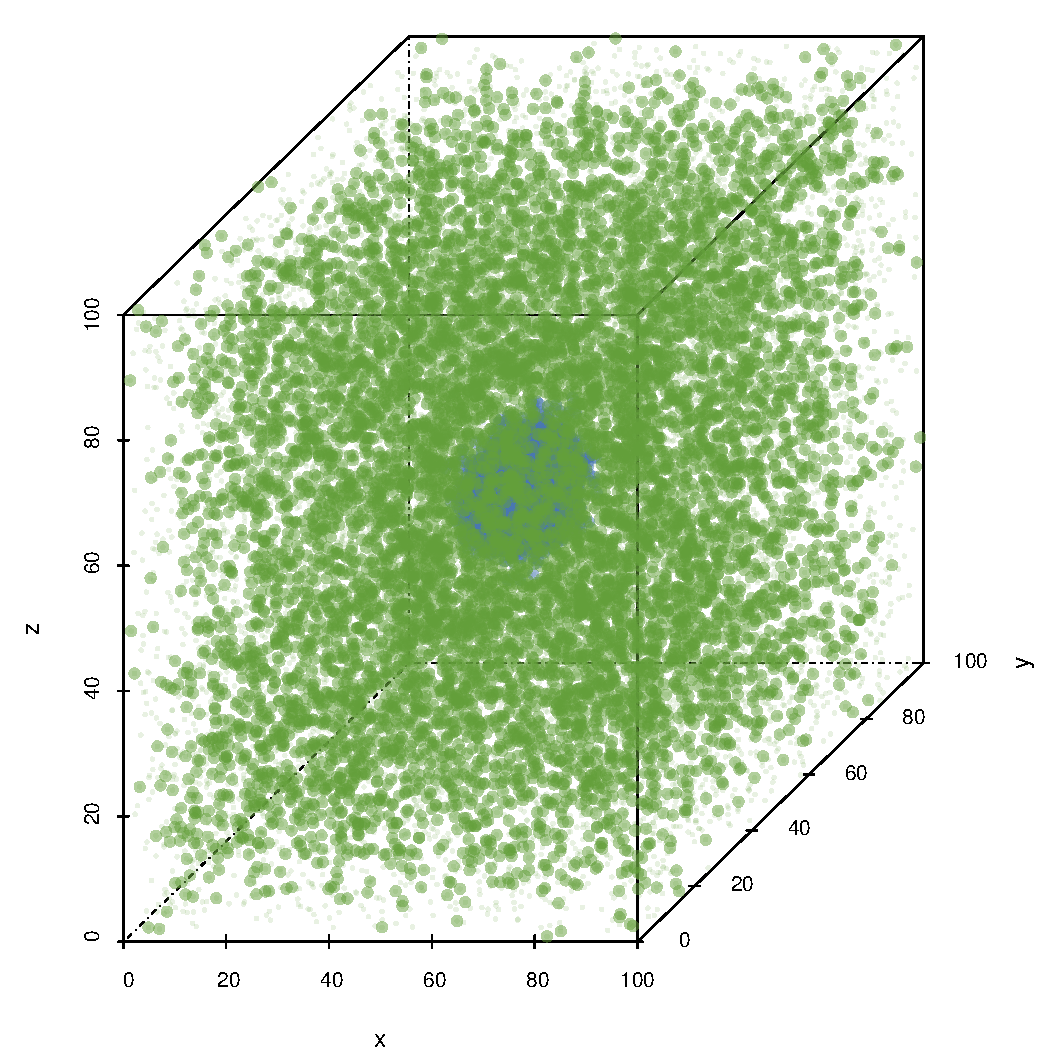
\includegraphics[keepaspectratio=true, width=\textwidth, height=0.23\textheight]{discussion/img/ferdosi_1_abs_error_mbeSmallerThansambe}
				\caption{Data set \ferdosiOne}
				\label{fig:discussion:performance:mbeLowerError:ferdosi1}
			\end{subfigure}
			\begin{subfigure}{0.23\textwidth}
				\centering
				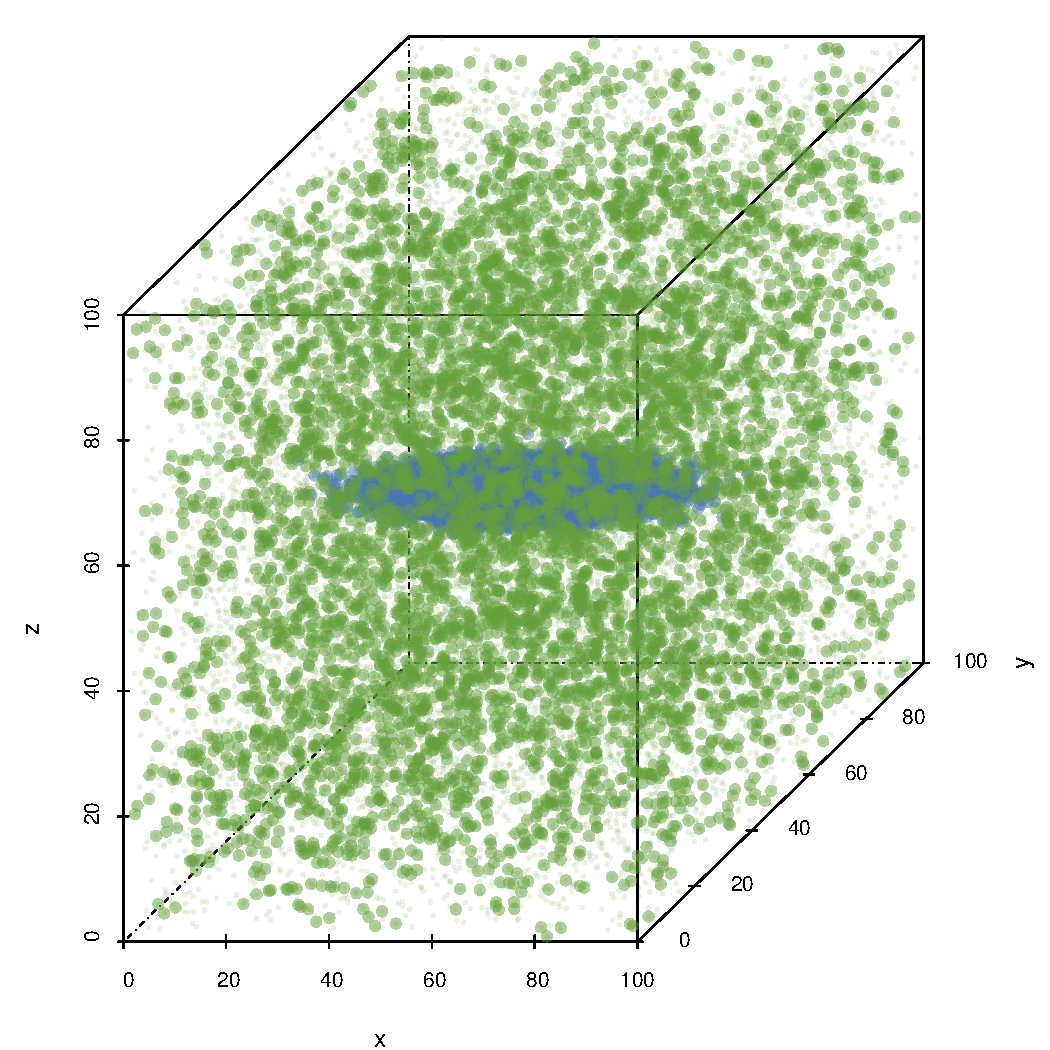
\includegraphics[keepaspectratio=true, width=\textwidth, height=0.23\textheight]{discussion/img/baakman_1_abs_error_mbeSmallerThansambe}
				\caption{Data set \baakmanOne}
				\label{fig:discussion:performance:mbeLowerError:baakman1}
			\end{subfigure}	
			\subfigvspace
			\begin{subfigure}{0.23\textwidth}
				\centering
				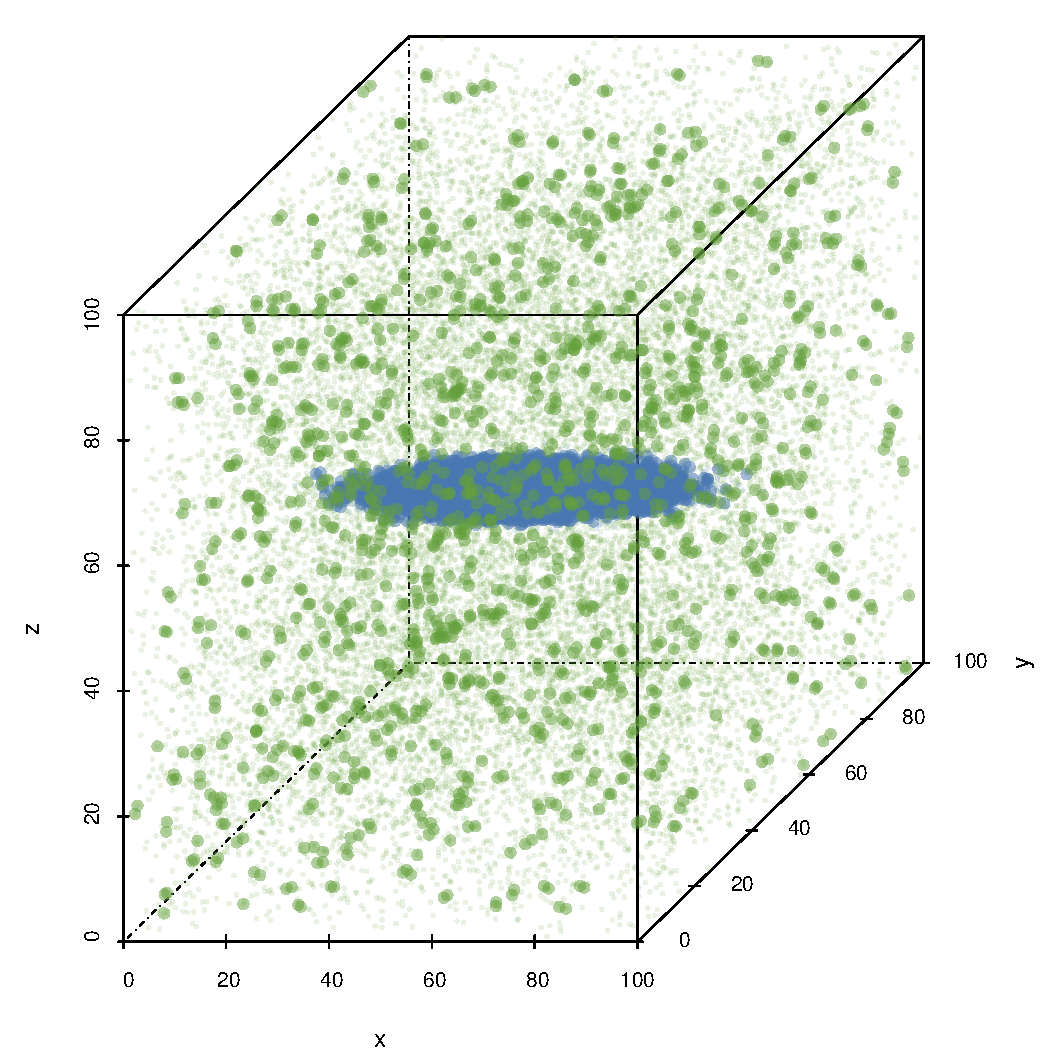
\includegraphics[keepaspectratio=true, width=\textwidth, height=0.23\textheight]{discussion/img/baakman_4_abs_error_mbeSmallerThansambe}
				\caption{Data set \baakmanFour}
				\label{fig:discussion:performance:mbeLowerError:baakman4}
			\end{subfigure}		
			\begin{subfigure}{0.23\textwidth}
				\centering
				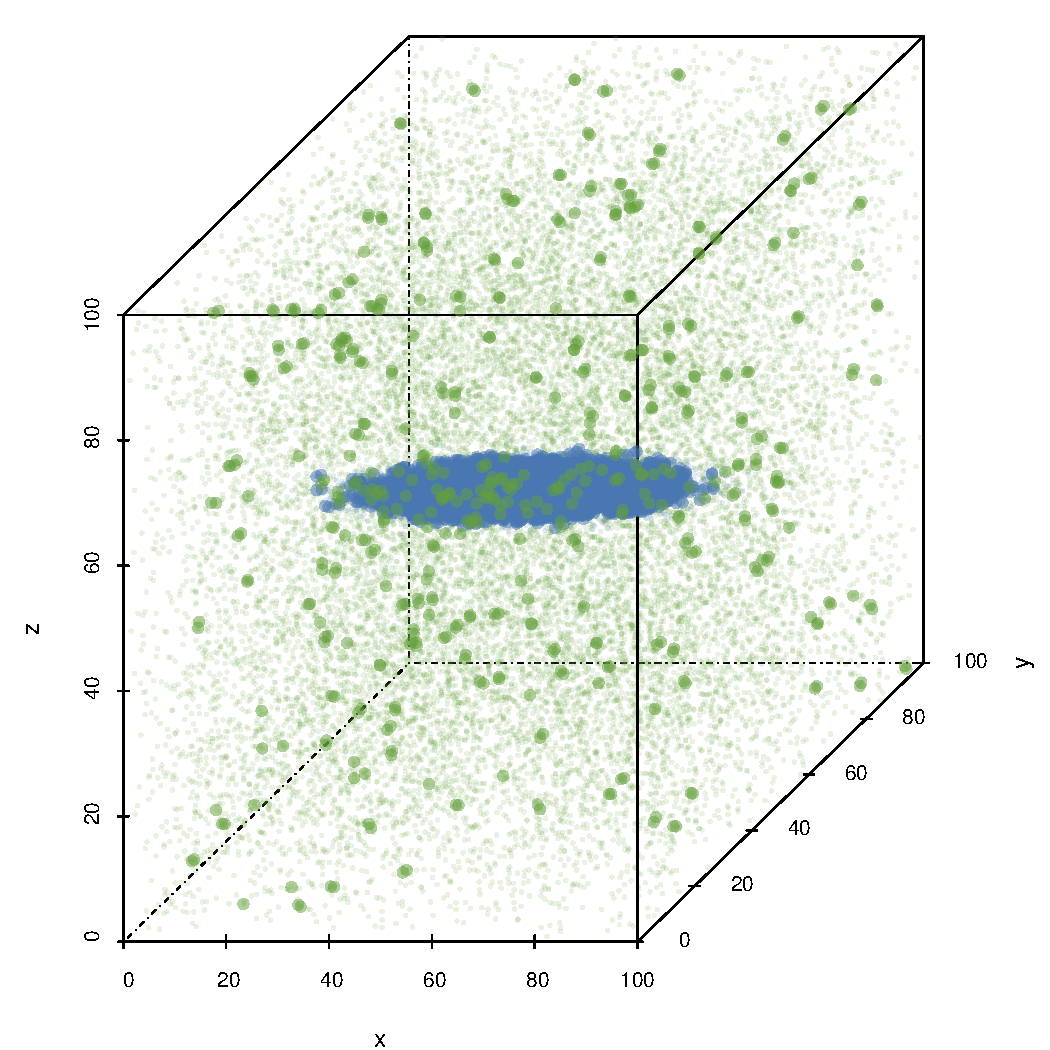
\includegraphics[keepaspectratio=true, width=\textwidth, height=0.23\textheight]{discussion/img/baakman_5_abs_error_mbeSmallerThansambe}
				\caption{Data set \baakmanFive}
				\label{fig:discussion:performance:mbeLowerError:baakman5}
			\end{subfigure}			
			\caption{Low opacity scatter plot of data set %
				\subref{fig:discussion:performance:mbeLowerError:ferdosi1} \ferdosiOne, %
				\subref{fig:discussion:performance:mbeLowerError:baakman1} \baakmanOne, %
				\subref{fig:discussion:performance:mbeLowerError:baakman4} \baakmanFour, and %
				\subref{fig:discussion:performance:mbeLowerError:baakman5} \baakmanFive, %
				with an overlay of larger, colored points where the absolute error of \sambe is larger than the absolute error of \mbe.}
			\label{fig:discussion:performance:singleSphere:mbeLowerError}
		\end{figure}
		%	
		The plots in \cref{fig:discussion:performance:singleSphere:mbeLowerError} emphasize the points in data set \ferdosiOne and \baakmanOne where the absolute error of \mbe is smaller than that of \sambe. These plots show that the shape-adaptive kernels outperform symmetric kernels near the borders of the data sets.
			% Why the boundary effect
			We expect that this boundary effect is due to the strong anisotropy of the local neighborhood of the points near the limits of the data sets. Consequently the domain of the shape-adaptive kernels extends less outside of the boundaries of the data set than the domains of the symmetric kernels. This results in less underestimation of densities near the boundary of the data set, if shape-adaptive kernels are used.
			% Why is it stonger of the Gaussian is more anisotropic
			Furthermore the strength of the boundary effect seems to increase as the Gaussian component of the data set is more anisotropic. However the seemingly better performance of \sambe is due to an increase in the number of points where the density estimated by \sambe equals the density estimated by \mbe. In data set \ferdosiOne the two estimators give a different result on all points. In data set \baakmanOne the estimators agree on the density of \percentage{1.327294605254362e+01} of the points, this increases to \percentage{3.535329901731399e+01} in data set \baakmanFive.
			%SAMBE == MBE
			%Ferdosi 1 (0.000000000000000e+00 percent)
			%Baakman 1 (1.327294605254362e+01 percent)
			%Baakman 4 (2.989838892974129e+01 percent)
			%Baakman 5 (3.535329901731399e+01 percent)
			As the Gaussian component becomes more anisotropic the number of points whose local neighborhood consists only of uniform noise increases. On average the covariance matrix of neighborhoods that contain primarily points sampled from the noise component should be scalar. Consequently as the anisotropy of the Gaussian component increases more shape-adaptive kernels take on a shape that is near-symmetric. This results in points were both estimators give the same approximated density. 
	
	% Multi Sphere
		\begin{figure}
			\centering
			\begin{subfigure}{0.23\textwidth}
				\centering
				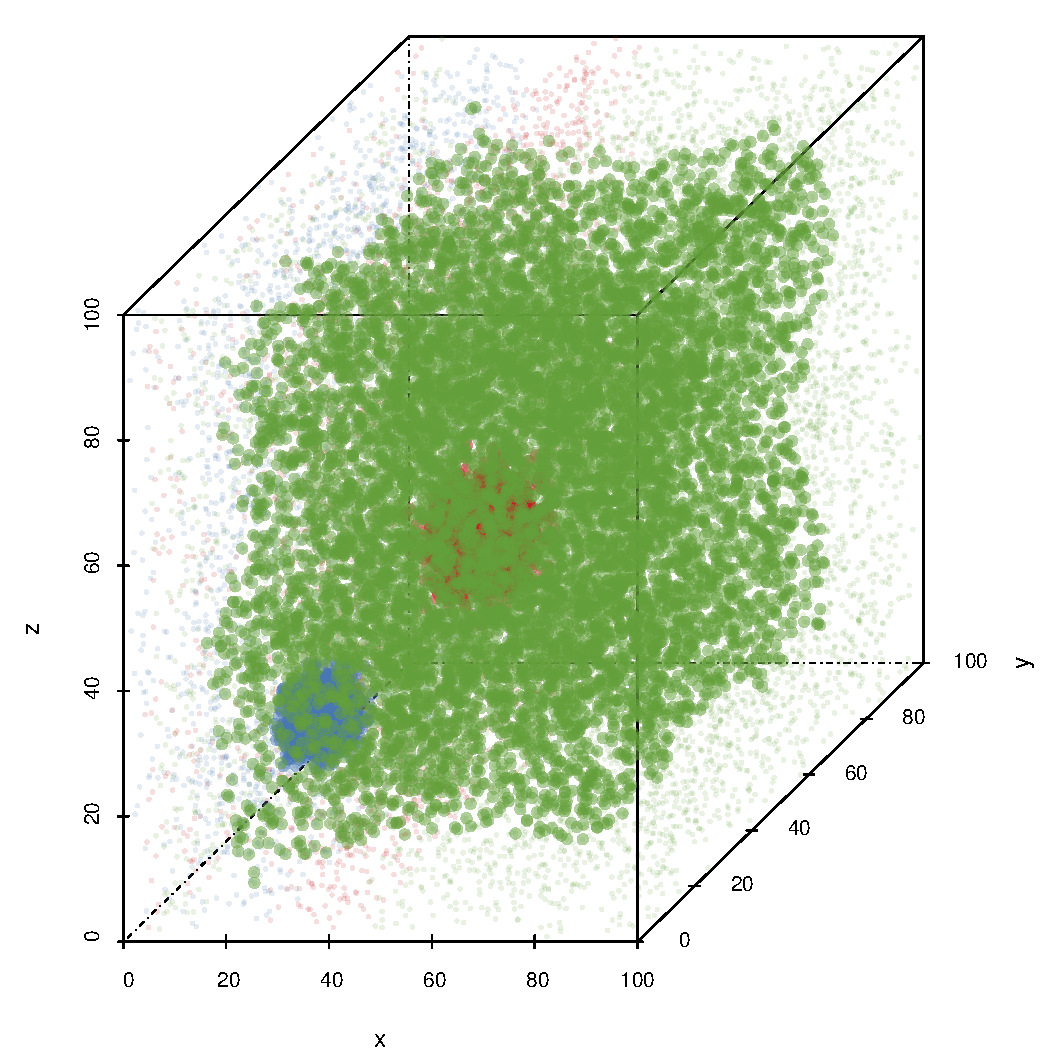
\includegraphics[keepaspectratio=true, width=\textwidth, height=0.23\textheight]{discussion/img/ferdosi_2_abs_error_mbeSmallerThansambe}
				\caption{Data set \ferdosiTwo}
				\label{fig:discussion:performance:mbeLowerError:ferdosi2}
			\end{subfigure}
			\begin{subfigure}{0.23\textwidth}
				\centering
				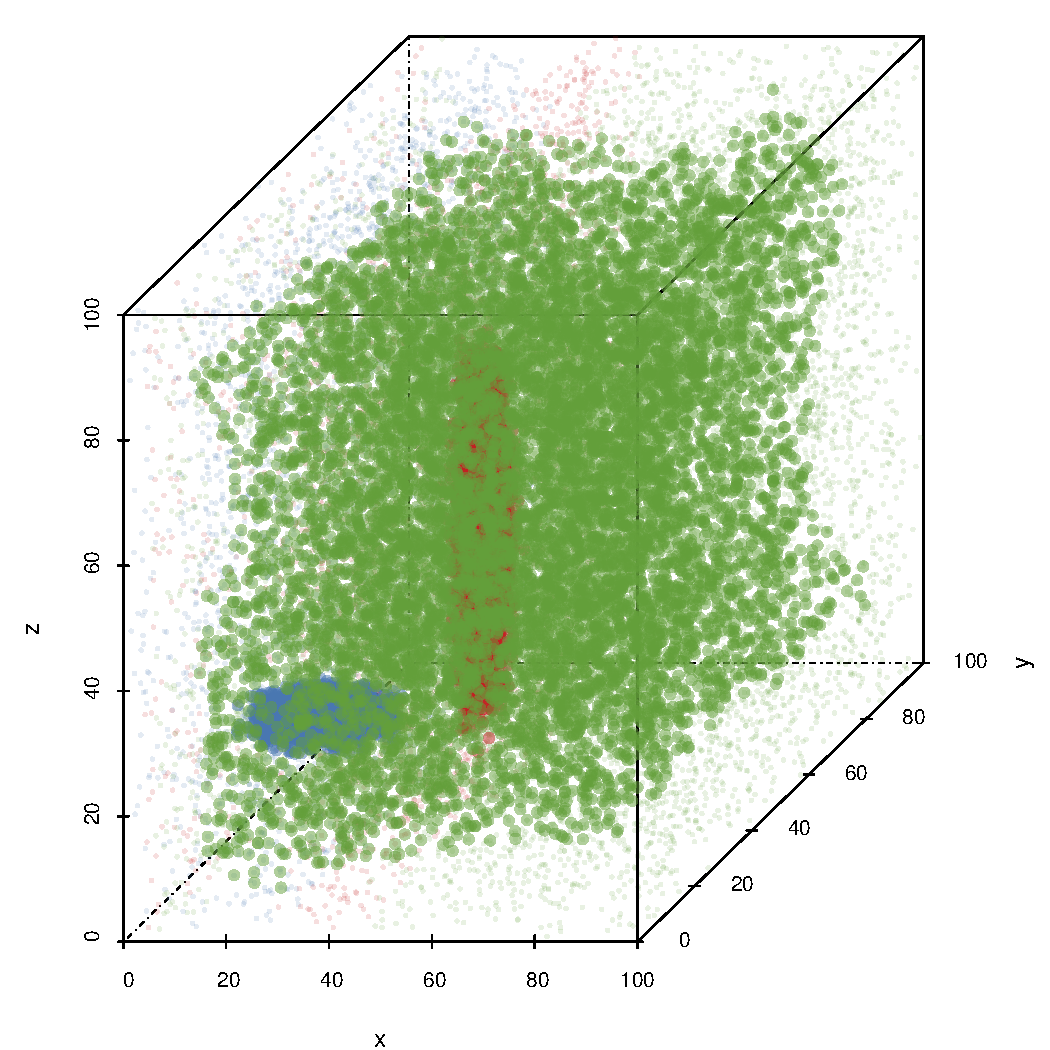
\includegraphics[keepaspectratio=true, width=\textwidth, height=0.23\textheight]{discussion/img/baakman_2_abs_error_mbeSmallerThansambe}
				\caption{Data set \baakmanTwo}
				\label{fig:discussion:performance:mbeLowerError:baakman2}
			\end{subfigure}	
			\subfigvspace
			\begin{subfigure}{0.23\textwidth}
				\centering
				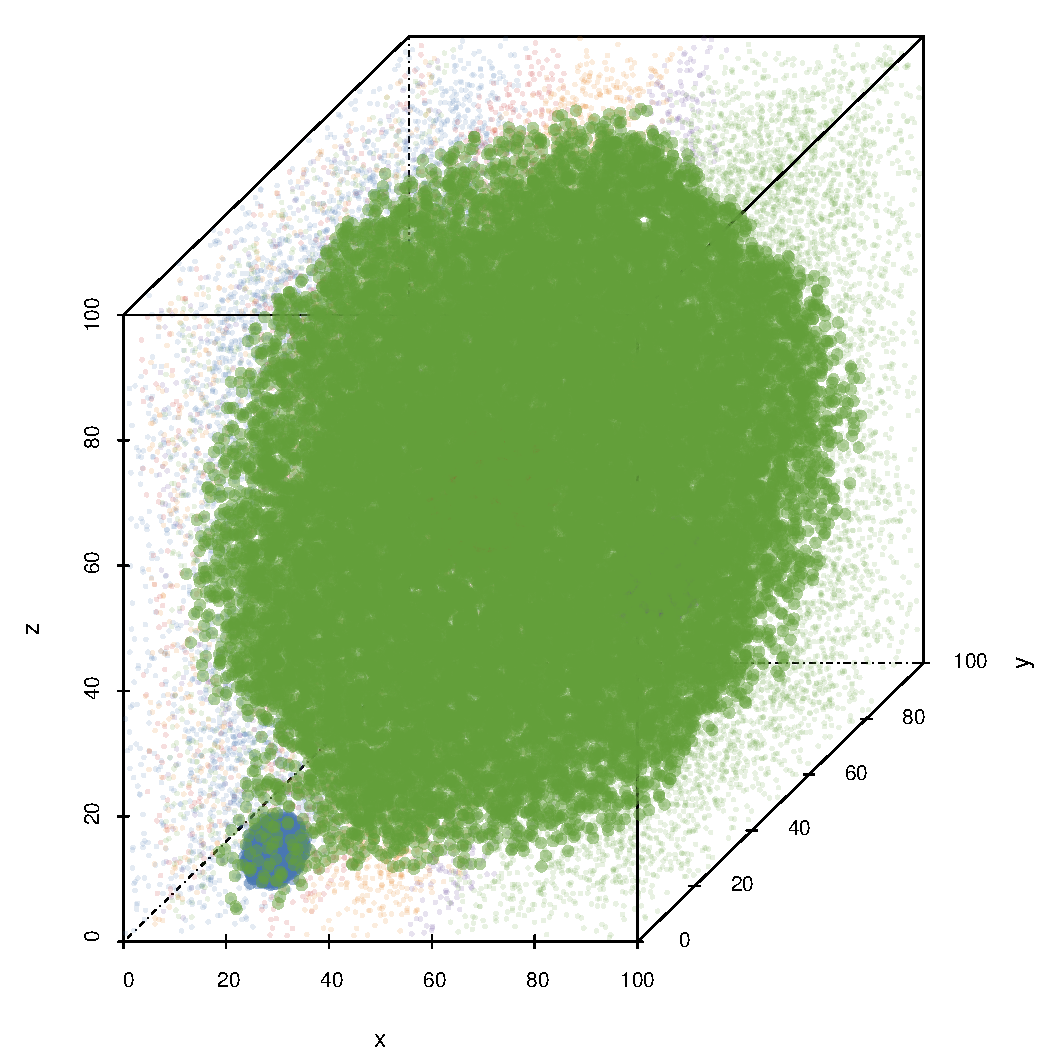
\includegraphics[keepaspectratio=true, width=\textwidth, height=0.23\textheight]{discussion/img/ferdosi_3_abs_error_mbeSmallerThansambe}
				\caption{Data set \ferdosiThree}
				\label{fig:discussion:performance:mbeLowerError:ferdosi3}
			\end{subfigure}
			\begin{subfigure}{0.23\textwidth}
				\centering
				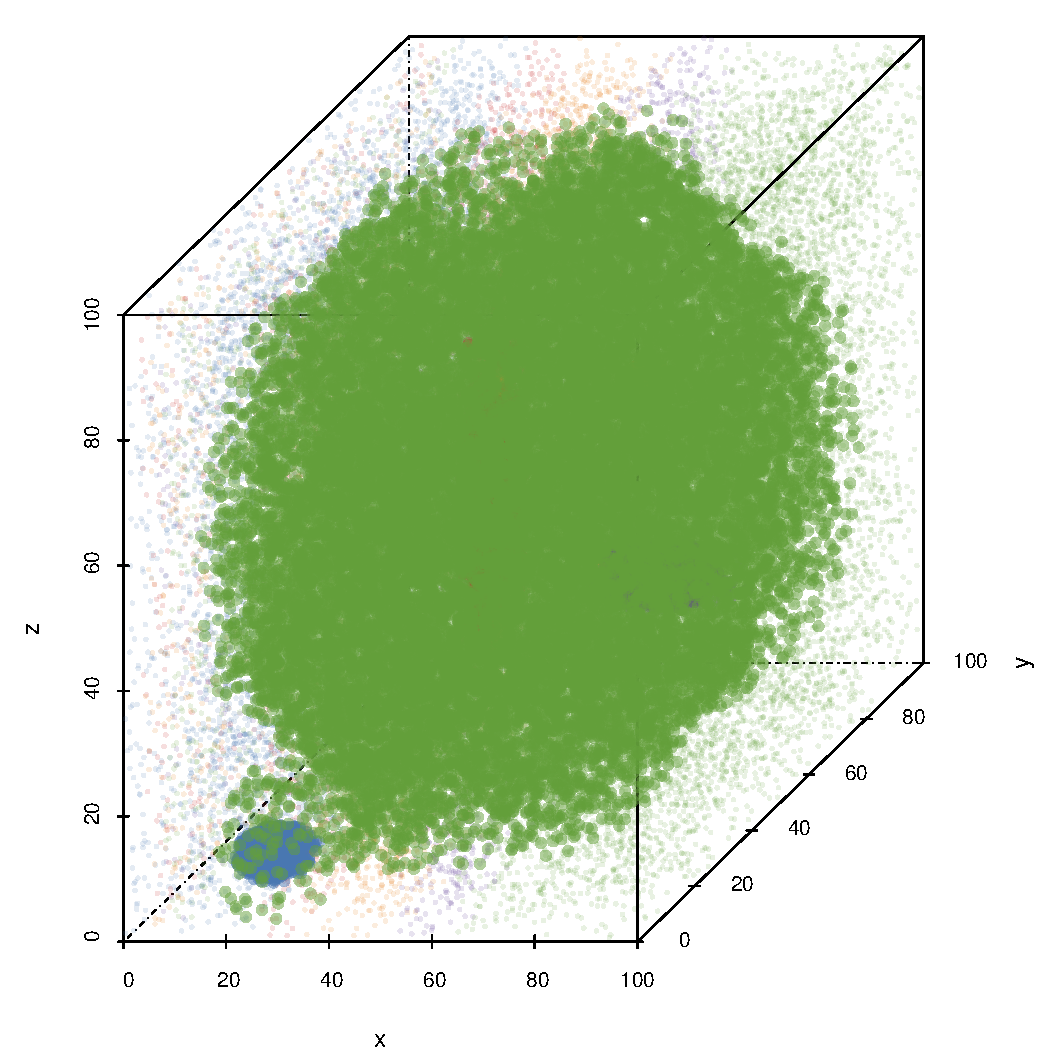
\includegraphics[keepaspectratio=true, width=\textwidth, height=0.23\textheight]{discussion/img/baakman_3_abs_error_mbeSmallerThansambe}
				\caption{Data set \baakmanThree}
				\label{fig:discussion:performance:mbeLowerError:baakman3}
			\end{subfigure}			
			\caption{Low opacity scatter plot of data set %
				\subref{fig:discussion:performance:mbeLowerError:ferdosi2} \ferdosiTwo, %
				\subref{fig:discussion:performance:mbeLowerError:baakman2} \baakmanTwo, %
				\subref{fig:discussion:performance:mbeLowerError:ferdosi3} \ferdosiThree, and %
				\subref{fig:discussion:performance:mbeLowerError:baakman3} \baakmanThree %
				with an overlay of high opacity, larger points where the absolute error of \mbe is smaller than that of \sambe.}
			\label{fig:discussion:performance:multisphere:mbeLowerError}
		\end{figure}	
		The points where using fixed-shape kernels results in a smaller error in data sets \ferdosiTwo through \baakmanThree are emphasized in
		\cref{fig:discussion:performance:multisphere:mbeLowerError}. We contribute the boundary effect in these data sets to the same cause as the boundary effect in the data sets with a single Gaussian component. Interestingly the points in data set \ferdosiThree and \baakmanThree where the absolute error of \mbe is lower, approximate a sphere, contrary to the cube they define for data set \ferdosiTwo and \baakmanTwo. It is our expectation that this is caused by the smaller distance between the means of the Gaussian components and the range of the uniform random background in \ferdosiThree and \baakmanThree.
			% Define Ferdosi 3 Noise
			To test this we define data set \ferdosiThreeNoise, which replaces the uniform random background of \ferdosiThree with $\uniformDist{[-20, -20, -20]}{[120, 120, 120]}$. We adjust the number of points sampled from this component to ensure that its density is equal to that of the noise component of \ferdosiThree.
			% Is there any effect on the MSE
			The overall \mse of both estimators is slightly smaller for data set \ferdosiThreeNoise than for \ferdosiThree, however the \mse of `Trivariate Gaussian 1' and 3 shows a small increase. 
			% Did the distance to the boundaries explain it?
			\Cref{fig:discussion:ferdosi3Noise:mbeLowerError} confirms that the spherical shape in \cref{fig:discussion:performance:mbeLowerError:ferdosi3,fig:discussion:performance:mbeLowerError:baakman3} is caused by the Gaussian near the boundary of the data set. As the shape defined by the emphasized points is now a cubical instead of spherical. 
			% The Plots of Ferdosi 3 Noise
			\begin{figure}
				\centering
				\begin{subfigure}{0.23\textwidth}
					\centering
					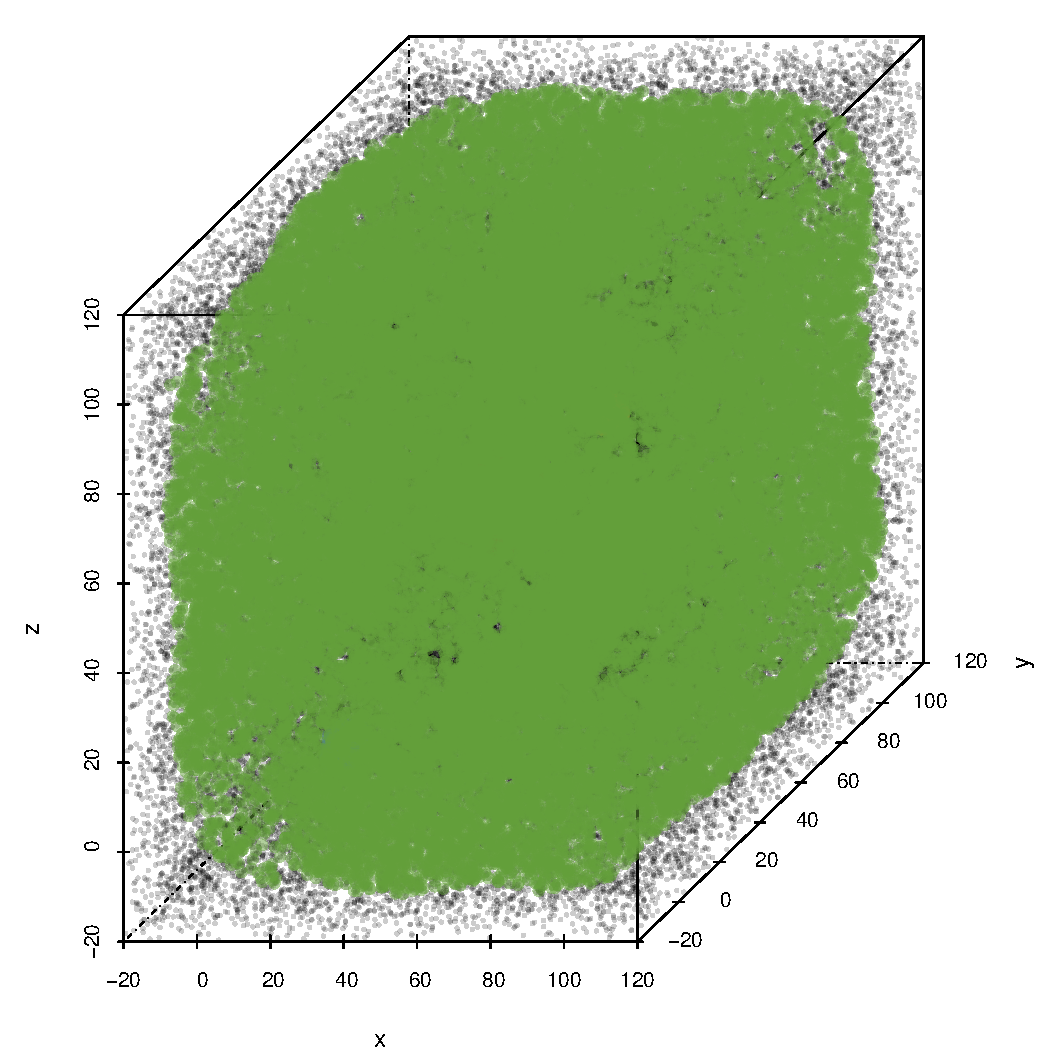
\includegraphics[keepaspectratio=true, width=\textwidth, height=0.23\textheight]{discussion/img/ferdosi_3_more_noise_abs_error_mbeSmallerThansambe.png}
					\caption{Absolute Error}
					\label{fig:discussion:ferdosi3Noise:mbeLowerError}
				\end{subfigure}		
				\begin{subfigure}{0.23\textwidth}
					\centering
					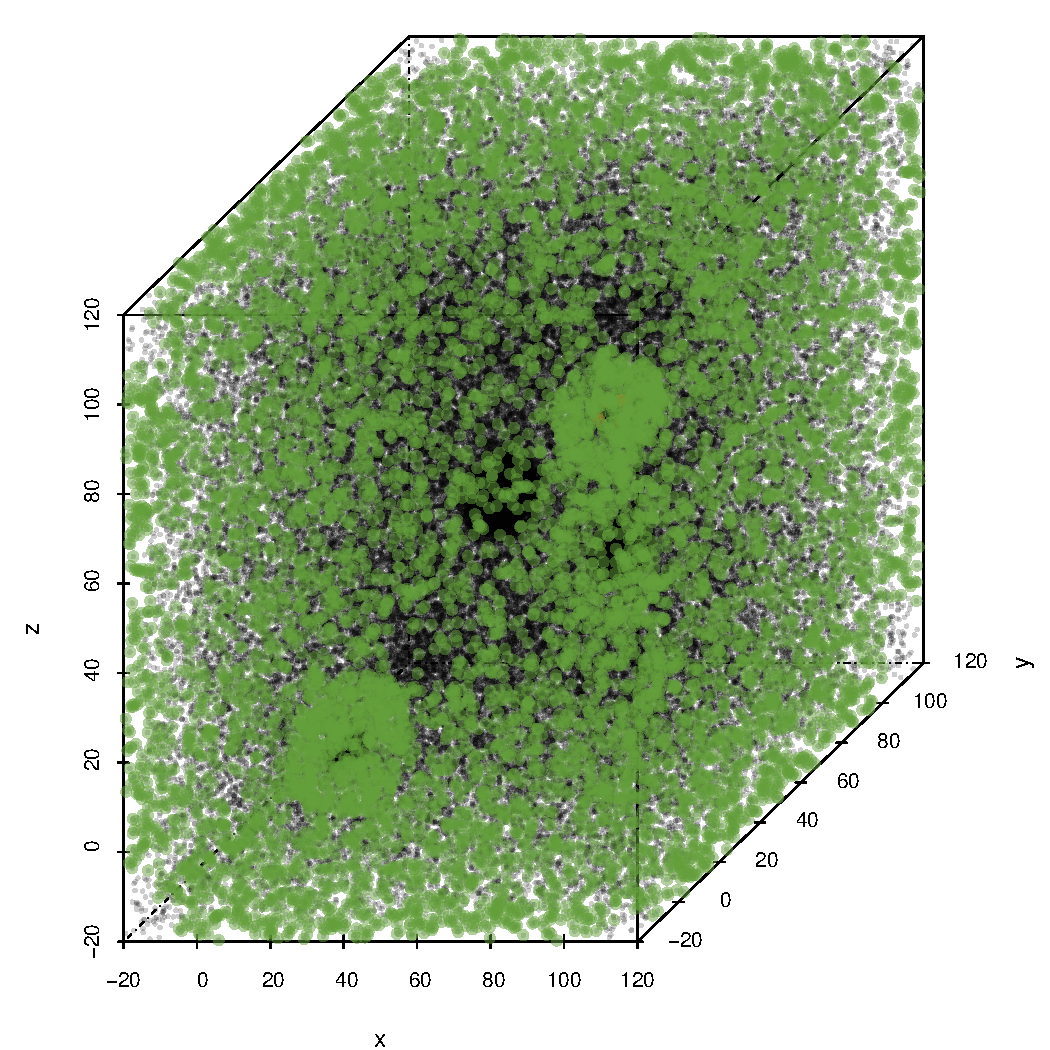
\includegraphics[keepaspectratio=true, width=\textwidth, height=0.23\textheight]{discussion/img/ferdosi_3_more_noise_anisotropy.png}
					\caption{Anisotropy}
					\label{fig:discussion:ferdosi3Noise:anisotropy}
				\end{subfigure}			
				\caption{Low opacity scatter plot of data set \ferdosiThreeNoise with %
					\subref{fig:discussion:ferdosi3Noise:mbeLowerError} points where the absolute error of \mbe is lower than that of \sambe and %
					\subref{fig:discussion:ferdosi3Noise:anisotropy} points sampled from the Gaussian components with kernels whose anisotropy falls in the \nth{95} percentile of the complete data set emphasized.}
				\label{fig:discussion:ferdosi3Noise}
			\end{figure}		

% Some conclusion
To conclude we have found that shape-adaptive kernels definitely improve performance in some cases, \ie near the boundary of the data sets and near the mean of some Gaussian components. Unfortunately in other cases the anisotropic kernels are detrimental. The difference in \mse between the two estimators shows that generally, using fixed-shape kernels is slightly advantageous. 

\subsection{Kernel Anisotropy}
\label{s:discussion:anisotropy}
%!TEX root = ../paper.tex

% Small differences in anisotropy  
	% Where are the differeneces largest -> plots
	% Refer to earlier solutions

% Highest anisotropy of noise component 
	% Kernel 'catches' spurious structures in noise -> increase K.

% 	  Denser component -> higher anisotropy of kernels
% AND Higher anistropy in component -> higer anisotropy in associated kernels
% AND Denser comonent -> lower MSE
	% Introduce the dataset A1 and A2, same anisotropy different density, what do we observe, what does it say about this correlation.

% Lack of difference in anisotropy between F3 and B3 in orange (‘Trivariate Gaussian 3’) component. 

We have found that near Gaussian components with a high volume eigensphere the kernels are too isotropic, whereas in the uniform random background fine structures are detected that result in too anisotropic kernels. Both of these problems might be solved by increasing the value of \KNNK. 
% Effect on noise:
We expect that increasing the size of the local neighborhood will decrease the number of detected fine structures. Which results in more isotropic kernels for points that lie in the uniform background.
% Effect on low density gaussians: 
Furthermore increasing the size of the local neighborhood might also allow the kernels to adapt their shape to nearby Gaussian components whose eigensphere has a high volume. Multiplying the \KNNK computed in \cref{eq:method:k} by ten, resulted in \sambe outperforming \mbe on dataset \baakmanFive. Furthermore the increased \KNNK also improved the performance on dataset \ferdosiThree, \baakmanThree and the datasets with a single Gaussian components. Whereas the performance of \sambe on dataset \ferdosiTwo and \baakmanTwo decreased. This suggest that blindly increasing the size of the local neighborhood will not consistently improve the performance of the estimator, but that same adaptive increase of \KNNK is required.

Another solution to the too anisotropic kernels in the noise might be to only use shape-adaptive kernels if the neighborhood is sufficiently anisotropic. One might even consider using a kernel-shape that is somewhere between the isotropic and the fully anisotropic kernel depending on the anisotropy of the local neighborhood. A difficulty with this approach is detecting the isotropy of the local neighborhood. As the obvious solution, the covariance matrix, has proven sensitive to fine structures within the noise. 

Finally the correlation between the performance of the estimators and the volume of the eigensphere of the Gaussian component suggests that the method used to compute the local bandwidths is far from ideal. 

\section{Discussion}
\label{s:discussion}
%!TEX root = ../paper.tex
This section discusses the previously presented results. We first consider the lack of difference in performance between the two estimators. The section after that is concerned with the anisotropy of the kernels used by the shape-adaptive estimator. Finally we offer some directions research into solving the identified issues might take.

\subsection{Performance}
\label{s:discussion:performance}
%!TEX root = ../paper.tex

% Hardly any difference between estimators
One of the most striking observations from \cref{s:results} is that the difference in performance between the two estimators is minimal. 
	
	% Study differences further mbe vs sambe plot
		% Single Sphere Sets
		Plotting the densities estimated by \sambe as a function of those estimated by \mbe shows no interesting differences between the two estimators for data set \ferdosiOne through \baakmanFive. 
		% Multi Sphere Sets
		However for data set \ferdosiTwo through \baakmanThree these plots reveal some differences between the estimators. As can be seen in \cref{fig:discussion:performance:two:mbevssambe}, using shape-adaptive kernels results in estimated densities that are generally higher than those estimated with a fixed-shape kernel for data set \ferdosiTwo and \baakmanTwo. Reviewing the raw data shows that \sambe underestimates densities less than \mbe on points near the mean of `Trivariate Gaussian 1'. The kernels in this neighborhood are all slightly anisotropic, which has allowed the shape-adaptive estimator to use more data points, to better approximate the local densities. Thus showing that estimating densities with shape-adaptive kernels can be advantageous.
		%
		\begin{figure}
			\centering
			\begin{subfigure}{0.3\textwidth}
				\centering
				\includegraphics[keepaspectratio=true, width=\textwidth, height=0.23\textheight]{discussion/img/ferdosi_2_60000_mbe_sambe.png}
				\caption{Data set \ferdosiTwo}
				\label{fig:discussion:performance:mbevssambe:ferdosi2}
			\end{subfigure}
			\subfigvspace
			\begin{subfigure}{0.3\textwidth}
				\centering
				\includegraphics[keepaspectratio=true, width=\textwidth, height=0.23\textheight]{discussion/img/baakman_2_60000_mbe_sambe.png}
				\caption{Data set \baakmanTwo}
				\label{fig:discussion:performance:mbevssambe:baakman2}
			\end{subfigure}	
			\caption{Plots of the densities estimated by \sambe as a function of those estimated by \mbe for data set %
				\subref{fig:discussion:performance:mbevssambe:ferdosi2} % 
				\ferdosiTwo and %
				\subref{fig:discussion:performance:mbevssambe:baakman2} %
				\baakmanTwo.
			}
			\label{fig:discussion:performance:two:mbevssambe}
		\end{figure}
		
		% Ferdosi 3 / Baakman 3
		\Cref{fig:discussion:performance:four:mbevssambe} shows the opposite effect; the densities estimated by \sambe for data set \ferdosiThree and \baakmanThree are generally lower than those estimated by \mbe. Reviewing the raw data shows that the points where the differences in estimated densities between the two estimators are largest lie near the mean of the `Trivariate Gaussian 3' in both data set \ferdosiThree and \baakmanThree. The number of points used in the density estimate by \sambe is consistently lower than the number of points used by the fixed-shape estimator. Given the relatively high anisotropy of the kernels in that area we expect that this is due to the kernels reflecting fine local structures, instead of the global neighborhood. 
		%	
		\begin{figure}
			\centering
			\begin{subfigure}{0.3\textwidth}
				\centering
				\includegraphics[keepaspectratio=true, width=\textwidth, height=0.23\textheight]{discussion/img/ferdosi_3_120000_mbe_sambe.png}
				\caption{Data set \ferdosiThree}
				\label{fig:discussion:performance:mbevssambe:ferdosi3}
			\end{subfigure}
			\subfigvspace
			\begin{subfigure}{0.3\textwidth}
				\centering
				\includegraphics[keepaspectratio=true, width=\textwidth, height=0.23\textheight]{discussion/img/baakman_3_120000_mbe_sambe.png}
				\caption{Data set \baakmanThree}
				\label{fig:discussion:performance:mbevssambe:baakman3}
			\end{subfigure}	
			\caption{Plots of the density estimated by \sambe as a function of those estimated by \mbe for data set %
				\subref{fig:discussion:performance:mbevssambe:ferdosi3} % 
				\ferdosiThree and %
				\subref{fig:discussion:performance:mbevssambe:baakman3} %
				\baakmanThree.
			}
			\label{fig:discussion:performance:four:mbevssambe}
		\end{figure}

	% Where are the differences largest -> plots
	% Single Sphere
		\begin{figure}
			\centering
			\begin{subfigure}{0.23\textwidth}
				\centering
				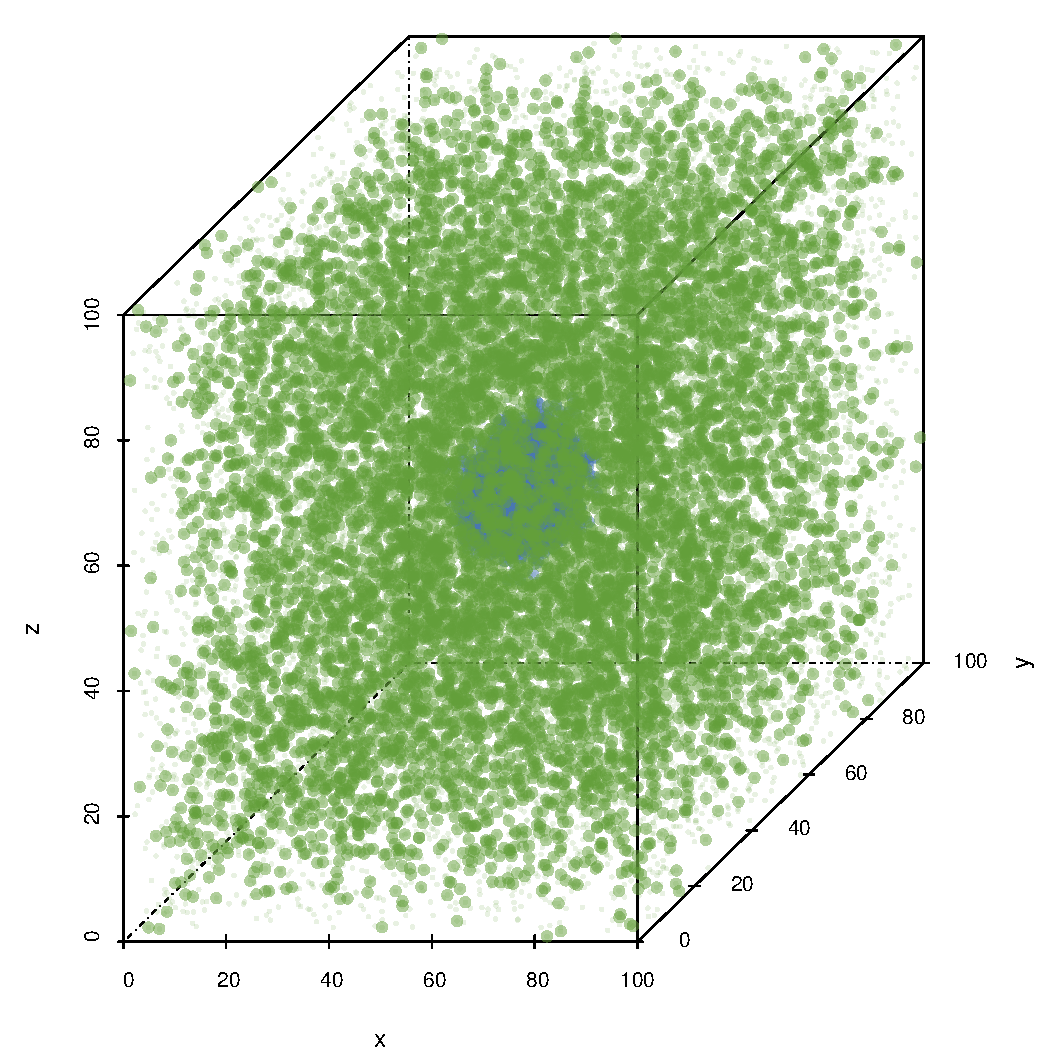
\includegraphics[keepaspectratio=true, width=\textwidth, height=0.23\textheight]{discussion/img/ferdosi_1_abs_error_mbeSmallerThansambe}
				\caption{Data set \ferdosiOne}
				\label{fig:discussion:performance:mbeLowerError:ferdosi1}
			\end{subfigure}
			\begin{subfigure}{0.23\textwidth}
				\centering
				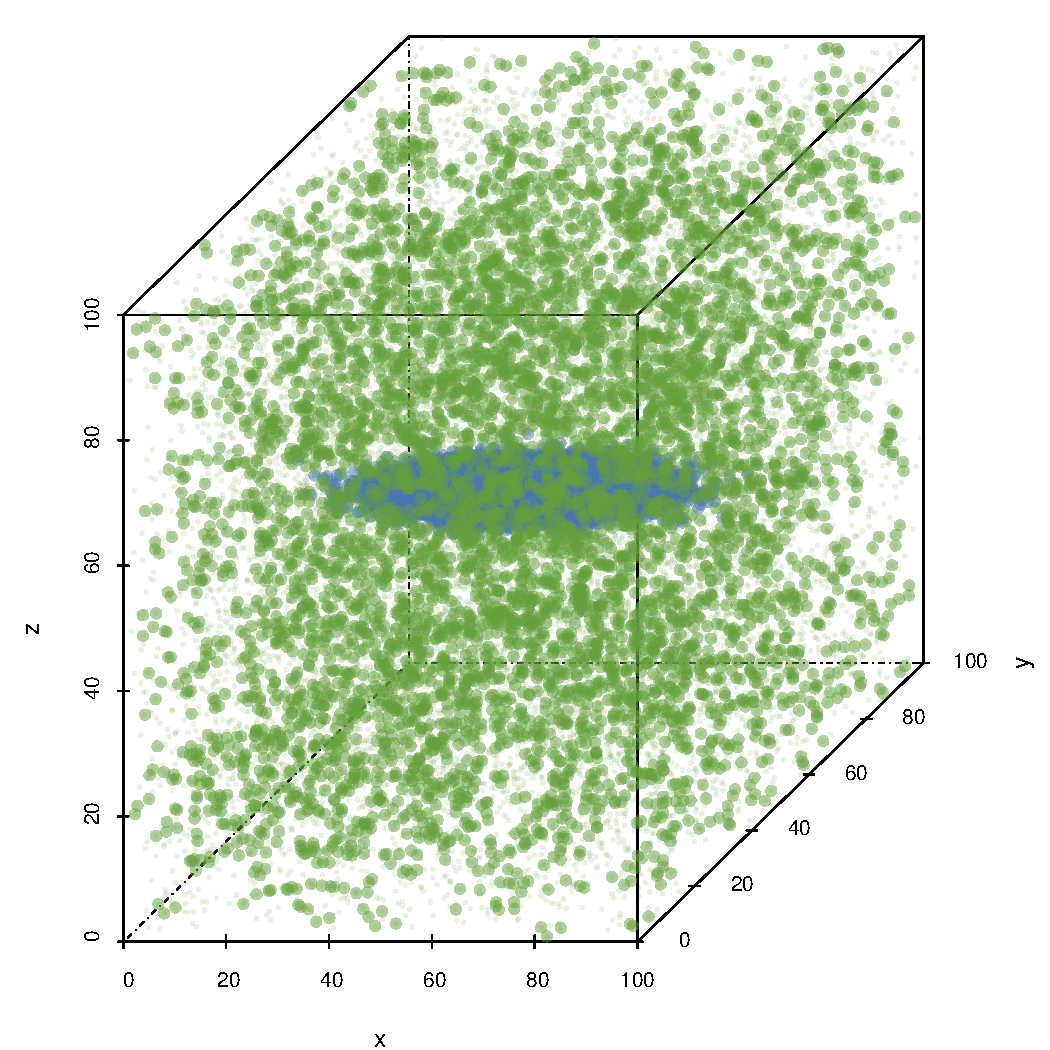
\includegraphics[keepaspectratio=true, width=\textwidth, height=0.23\textheight]{discussion/img/baakman_1_abs_error_mbeSmallerThansambe}
				\caption{Data set \baakmanOne}
				\label{fig:discussion:performance:mbeLowerError:baakman1}
			\end{subfigure}	
			\subfigvspace
			\begin{subfigure}{0.23\textwidth}
				\centering
				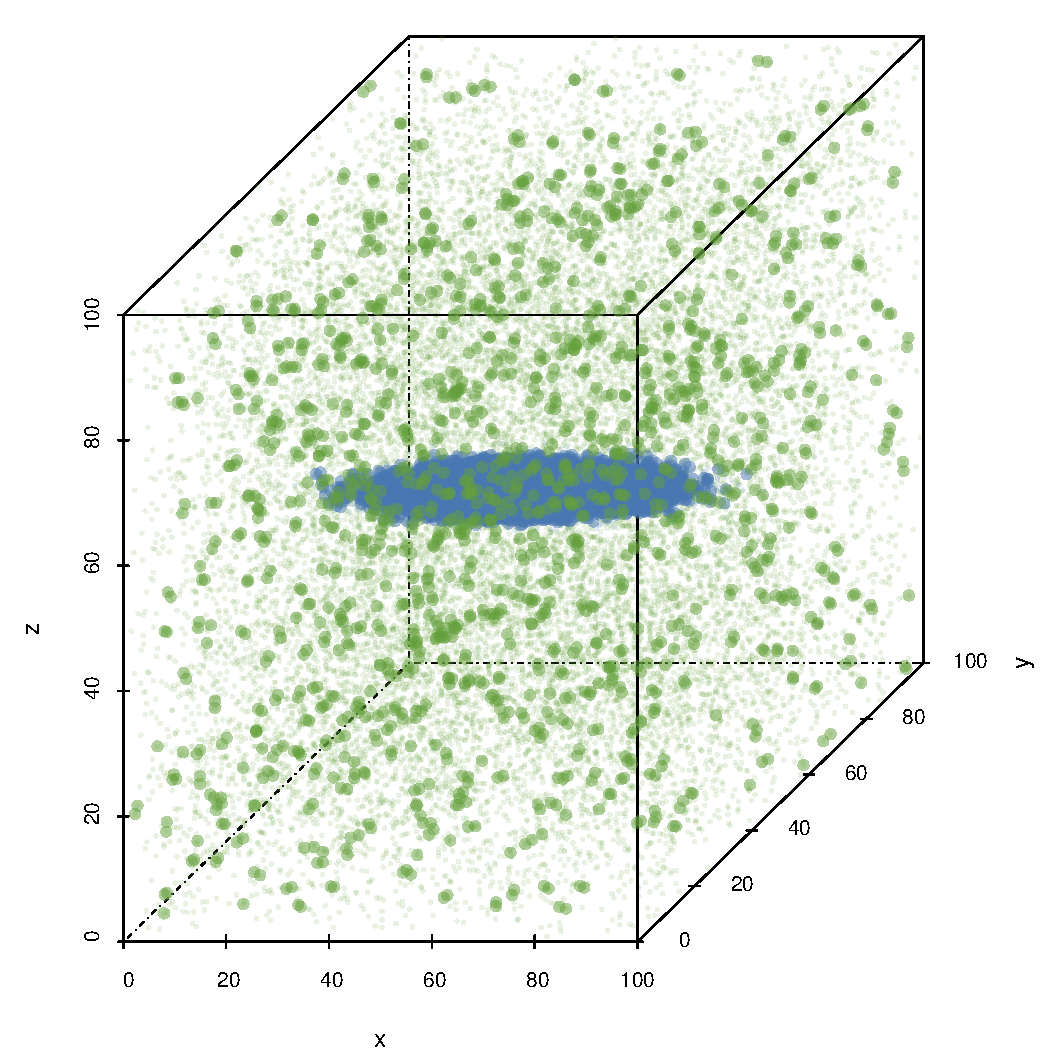
\includegraphics[keepaspectratio=true, width=\textwidth, height=0.23\textheight]{discussion/img/baakman_4_abs_error_mbeSmallerThansambe}
				\caption{Data set \baakmanFour}
				\label{fig:discussion:performance:mbeLowerError:baakman4}
			\end{subfigure}		
			\begin{subfigure}{0.23\textwidth}
				\centering
				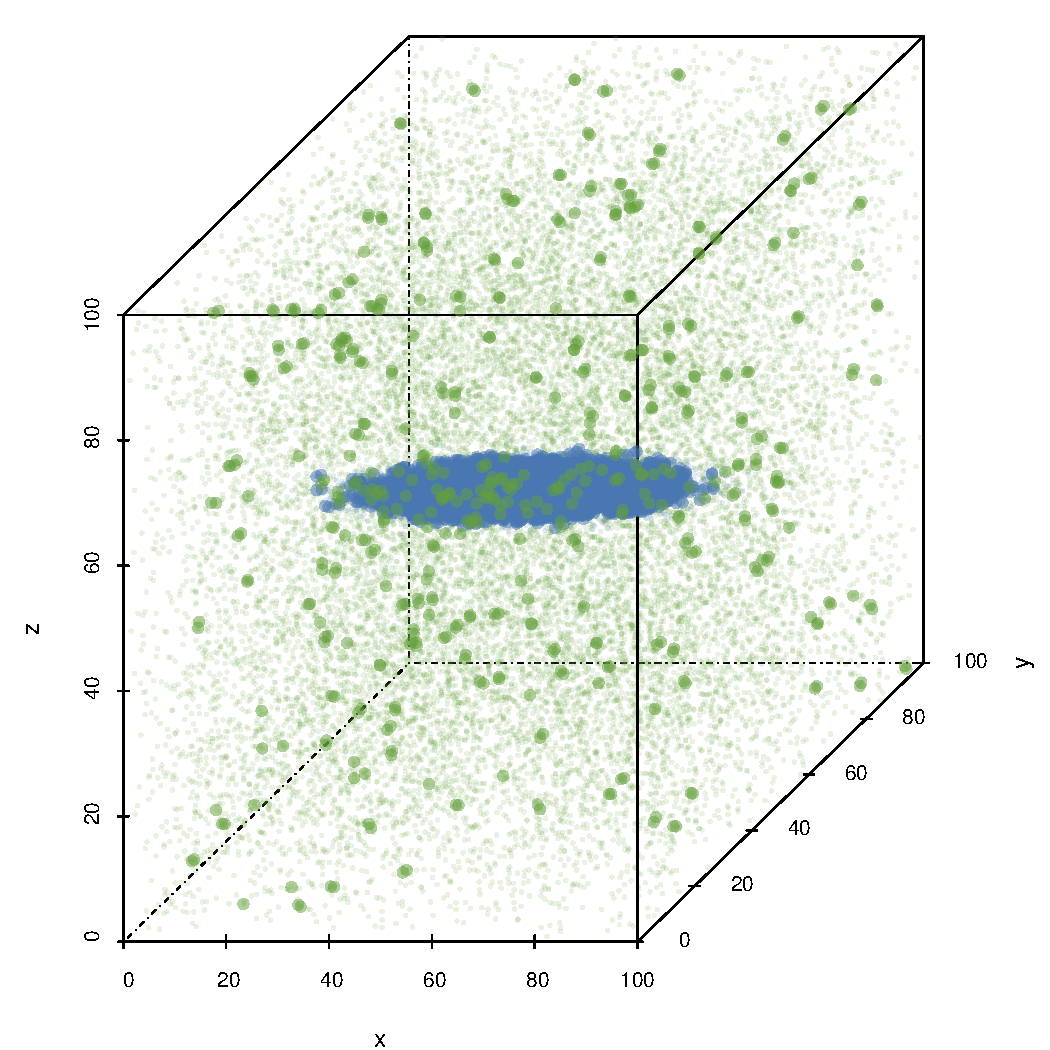
\includegraphics[keepaspectratio=true, width=\textwidth, height=0.23\textheight]{discussion/img/baakman_5_abs_error_mbeSmallerThansambe}
				\caption{Data set \baakmanFive}
				\label{fig:discussion:performance:mbeLowerError:baakman5}
			\end{subfigure}			
			\caption{Low opacity scatter plot of data set %
				\subref{fig:discussion:performance:mbeLowerError:ferdosi1} \ferdosiOne, %
				\subref{fig:discussion:performance:mbeLowerError:baakman1} \baakmanOne, %
				\subref{fig:discussion:performance:mbeLowerError:baakman4} \baakmanFour, and %
				\subref{fig:discussion:performance:mbeLowerError:baakman5} \baakmanFive, %
				with an overlay of larger, colored points where the absolute error of \sambe is larger than the absolute error of \mbe.}
			\label{fig:discussion:performance:singleSphere:mbeLowerError}
		\end{figure}
		%	
		The plots in \cref{fig:discussion:performance:singleSphere:mbeLowerError} emphasize the points in data set \ferdosiOne and \baakmanOne where the absolute error of \mbe is smaller than that of \sambe. These plots show that the shape-adaptive kernels outperform symmetric kernels near the borders of the data sets.
			% Why the boundary effect
			We expect that this boundary effect is due to the strong anisotropy of the local neighborhood of the points near the limits of the data sets. Consequently the domain of the shape-adaptive kernels extends less outside of the boundaries of the data set than the domains of the symmetric kernels. This results in less underestimation of densities near the boundary of the data set, if shape-adaptive kernels are used.
			% Why is it stonger of the Gaussian is more anisotropic
			Furthermore the strength of the boundary effect seems to increase as the Gaussian component of the data set is more anisotropic. However the seemingly better performance of \sambe is due to an increase in the number of points where the density estimated by \sambe equals the density estimated by \mbe. In data set \ferdosiOne the two estimators give a different result on all points. In data set \baakmanOne the estimators agree on the density of \percentage{1.327294605254362e+01} of the points, this increases to \percentage{3.535329901731399e+01} in data set \baakmanFive.
			%SAMBE == MBE
			%Ferdosi 1 (0.000000000000000e+00 percent)
			%Baakman 1 (1.327294605254362e+01 percent)
			%Baakman 4 (2.989838892974129e+01 percent)
			%Baakman 5 (3.535329901731399e+01 percent)
			As the Gaussian component becomes more anisotropic the number of points whose local neighborhood consists only of uniform noise increases. On average the covariance matrix of neighborhoods that contain primarily points sampled from the noise component should be scalar. Consequently as the anisotropy of the Gaussian component increases more shape-adaptive kernels take on a shape that is near-symmetric. This results in points were both estimators give the same approximated density. 
	
	% Multi Sphere
		\begin{figure}
			\centering
			\begin{subfigure}{0.23\textwidth}
				\centering
				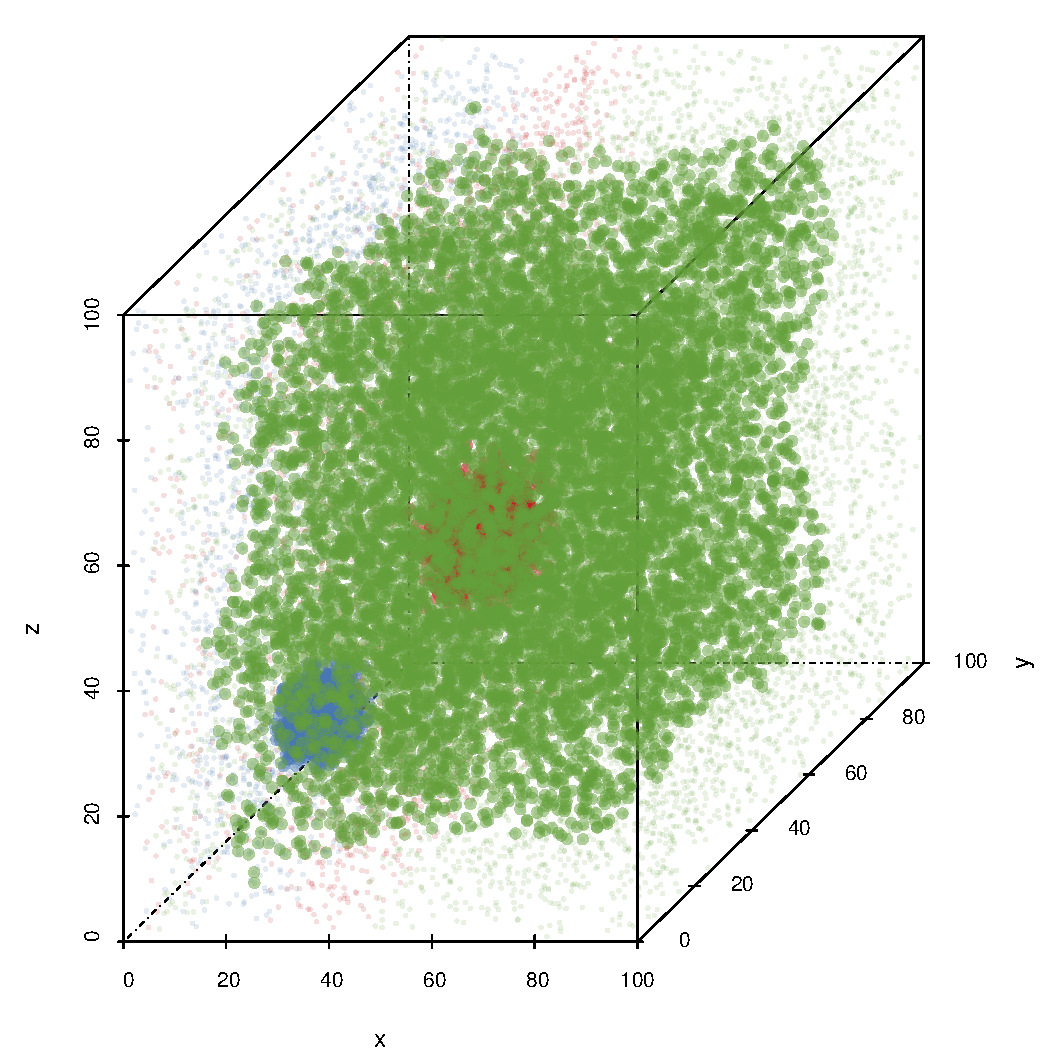
\includegraphics[keepaspectratio=true, width=\textwidth, height=0.23\textheight]{discussion/img/ferdosi_2_abs_error_mbeSmallerThansambe}
				\caption{Data set \ferdosiTwo}
				\label{fig:discussion:performance:mbeLowerError:ferdosi2}
			\end{subfigure}
			\begin{subfigure}{0.23\textwidth}
				\centering
				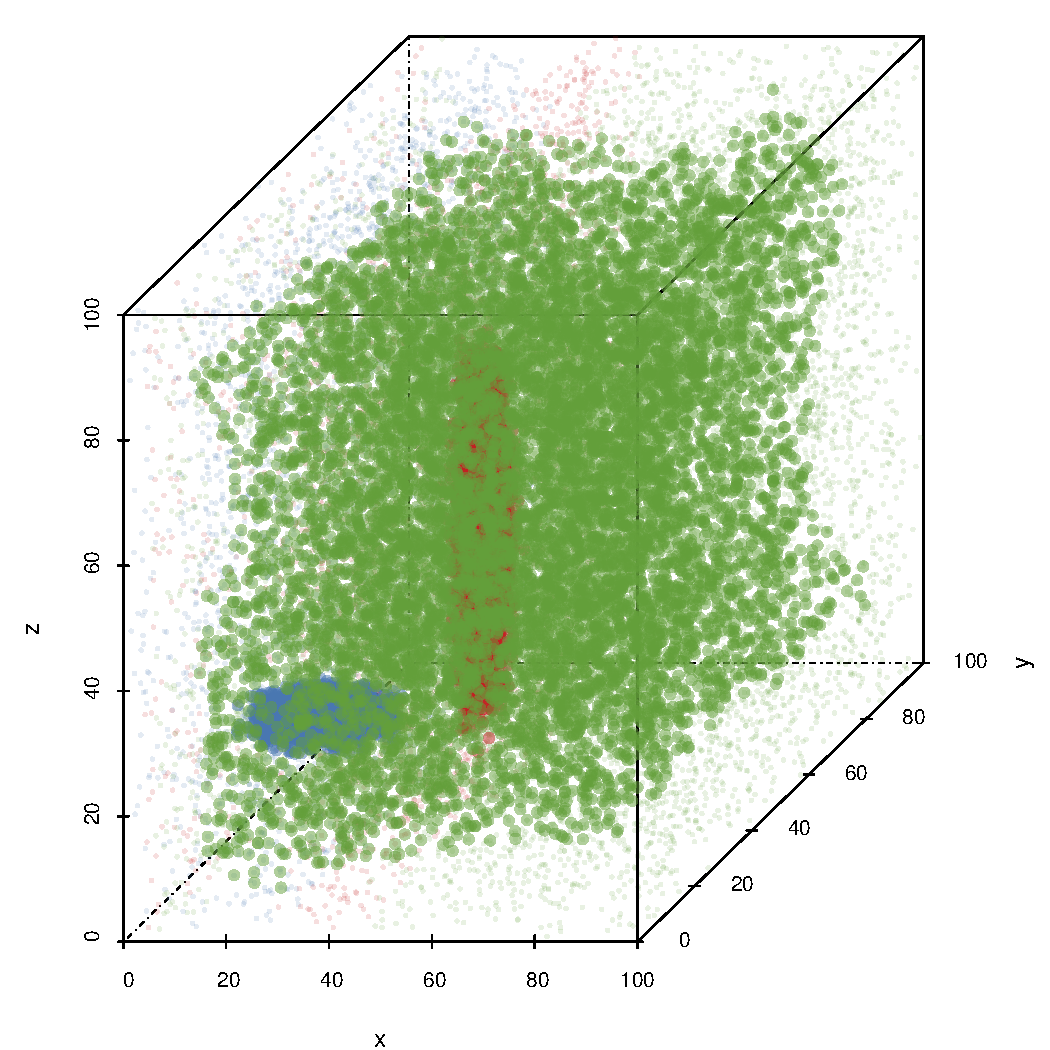
\includegraphics[keepaspectratio=true, width=\textwidth, height=0.23\textheight]{discussion/img/baakman_2_abs_error_mbeSmallerThansambe}
				\caption{Data set \baakmanTwo}
				\label{fig:discussion:performance:mbeLowerError:baakman2}
			\end{subfigure}	
			\subfigvspace
			\begin{subfigure}{0.23\textwidth}
				\centering
				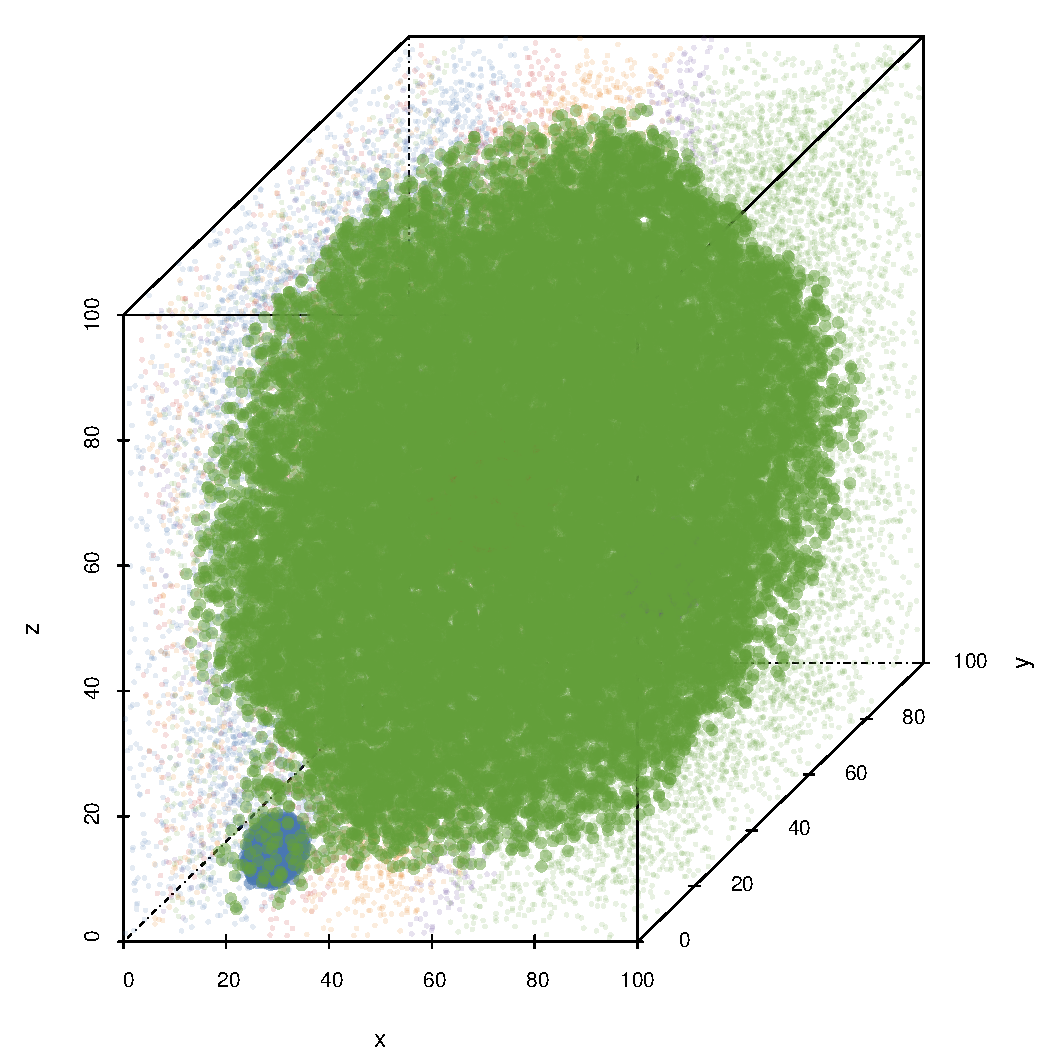
\includegraphics[keepaspectratio=true, width=\textwidth, height=0.23\textheight]{discussion/img/ferdosi_3_abs_error_mbeSmallerThansambe}
				\caption{Data set \ferdosiThree}
				\label{fig:discussion:performance:mbeLowerError:ferdosi3}
			\end{subfigure}
			\begin{subfigure}{0.23\textwidth}
				\centering
				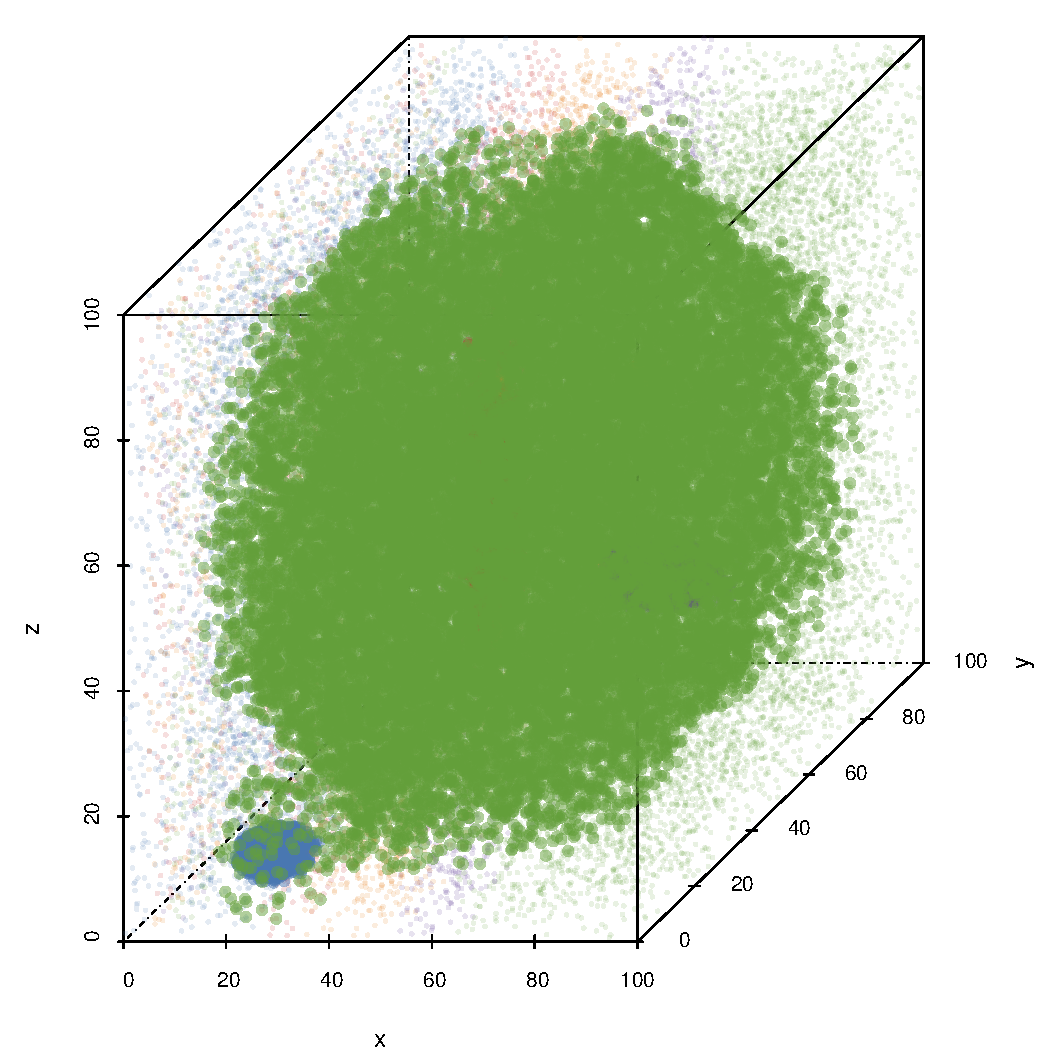
\includegraphics[keepaspectratio=true, width=\textwidth, height=0.23\textheight]{discussion/img/baakman_3_abs_error_mbeSmallerThansambe}
				\caption{Data set \baakmanThree}
				\label{fig:discussion:performance:mbeLowerError:baakman3}
			\end{subfigure}			
			\caption{Low opacity scatter plot of data set %
				\subref{fig:discussion:performance:mbeLowerError:ferdosi2} \ferdosiTwo, %
				\subref{fig:discussion:performance:mbeLowerError:baakman2} \baakmanTwo, %
				\subref{fig:discussion:performance:mbeLowerError:ferdosi3} \ferdosiThree, and %
				\subref{fig:discussion:performance:mbeLowerError:baakman3} \baakmanThree %
				with an overlay of high opacity, larger points where the absolute error of \mbe is smaller than that of \sambe.}
			\label{fig:discussion:performance:multisphere:mbeLowerError}
		\end{figure}	
		The points where using fixed-shape kernels results in a smaller error in data sets \ferdosiTwo through \baakmanThree are emphasized in
		\cref{fig:discussion:performance:multisphere:mbeLowerError}. We contribute the boundary effect in these data sets to the same cause as the boundary effect in the data sets with a single Gaussian component. Interestingly the points in data set \ferdosiThree and \baakmanThree where the absolute error of \mbe is lower, approximate a sphere, contrary to the cube they define for data set \ferdosiTwo and \baakmanTwo. It is our expectation that this is caused by the smaller distance between the means of the Gaussian components and the range of the uniform random background in \ferdosiThree and \baakmanThree.
			% Define Ferdosi 3 Noise
			To test this we define data set \ferdosiThreeNoise, which replaces the uniform random background of \ferdosiThree with $\uniformDist{[-20, -20, -20]}{[120, 120, 120]}$. We adjust the number of points sampled from this component to ensure that its density is equal to that of the noise component of \ferdosiThree.
			% Is there any effect on the MSE
			The overall \mse of both estimators is slightly smaller for data set \ferdosiThreeNoise than for \ferdosiThree, however the \mse of `Trivariate Gaussian 1' and 3 shows a small increase. 
			% Did the distance to the boundaries explain it?
			\Cref{fig:discussion:ferdosi3Noise:mbeLowerError} confirms that the spherical shape in \cref{fig:discussion:performance:mbeLowerError:ferdosi3,fig:discussion:performance:mbeLowerError:baakman3} is caused by the Gaussian near the boundary of the data set. As the shape defined by the emphasized points is now a cubical instead of spherical. 
			% The Plots of Ferdosi 3 Noise
			\begin{figure}
				\centering
				\begin{subfigure}{0.23\textwidth}
					\centering
					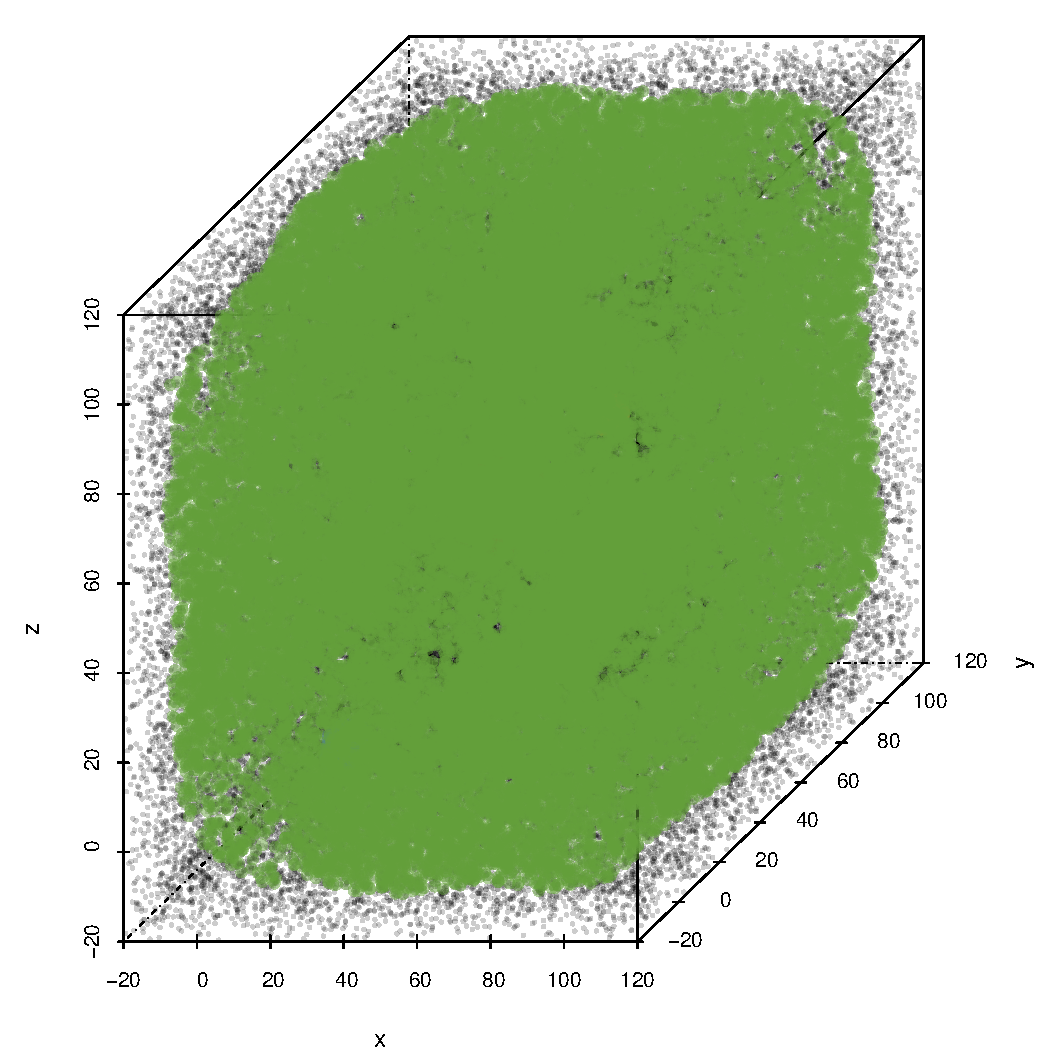
\includegraphics[keepaspectratio=true, width=\textwidth, height=0.23\textheight]{discussion/img/ferdosi_3_more_noise_abs_error_mbeSmallerThansambe.png}
					\caption{Absolute Error}
					\label{fig:discussion:ferdosi3Noise:mbeLowerError}
				\end{subfigure}		
				\begin{subfigure}{0.23\textwidth}
					\centering
					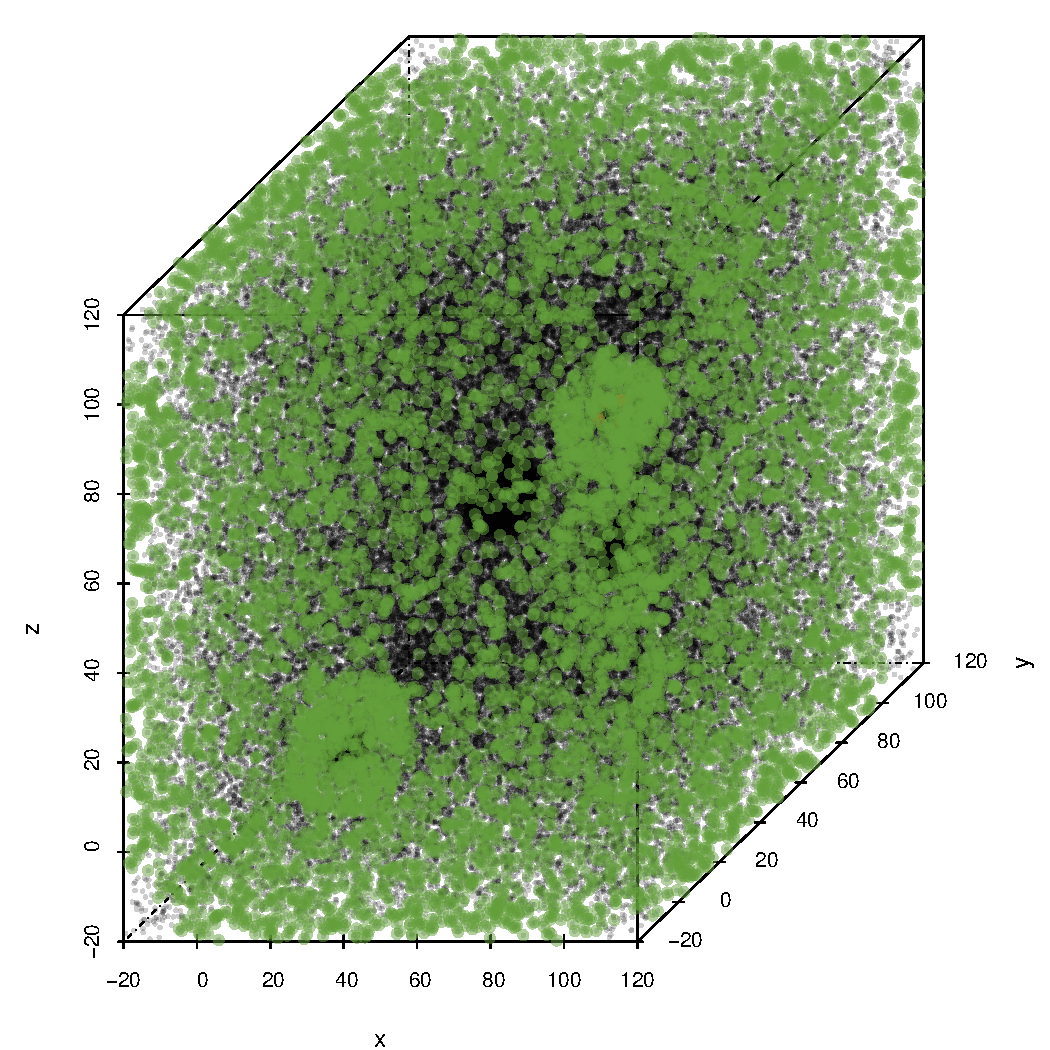
\includegraphics[keepaspectratio=true, width=\textwidth, height=0.23\textheight]{discussion/img/ferdosi_3_more_noise_anisotropy.png}
					\caption{Anisotropy}
					\label{fig:discussion:ferdosi3Noise:anisotropy}
				\end{subfigure}			
				\caption{Low opacity scatter plot of data set \ferdosiThreeNoise with %
					\subref{fig:discussion:ferdosi3Noise:mbeLowerError} points where the absolute error of \mbe is lower than that of \sambe and %
					\subref{fig:discussion:ferdosi3Noise:anisotropy} points sampled from the Gaussian components with kernels whose anisotropy falls in the \nth{95} percentile of the complete data set emphasized.}
				\label{fig:discussion:ferdosi3Noise}
			\end{figure}		

% Some conclusion
To conclude we have found that shape-adaptive kernels definitely improve performance in some cases, \ie near the boundary of the data sets and near the mean of some Gaussian components. Unfortunately in other cases the anisotropic kernels are detrimental. The difference in \mse between the two estimators shows that generally, using fixed-shape kernels is slightly advantageous. 

\subsection{Kernel Anisotropy}
\label{s:discussion:anisotropy}
%!TEX root = ../paper.tex

% Small differences in anisotropy  
	% Where are the differeneces largest -> plots
	% Refer to earlier solutions

% Highest anisotropy of noise component 
	% Kernel 'catches' spurious structures in noise -> increase K.

% 	  Denser component -> higher anisotropy of kernels
% AND Higher anistropy in component -> higer anisotropy in associated kernels
% AND Denser comonent -> lower MSE
	% Introduce the dataset A1 and A2, same anisotropy different density, what do we observe, what does it say about this correlation.

% Lack of difference in anisotropy between F3 and B3 in orange (‘Trivariate Gaussian 3’) component. 

We have found that near Gaussian components with a high volume eigensphere the kernels are too isotropic, whereas in the uniform random background fine structures are detected that result in too anisotropic kernels. Both of these problems might be solved by increasing the value of \KNNK. 
% Effect on noise:
We expect that increasing the size of the local neighborhood will decrease the number of detected fine structures. Which results in more isotropic kernels for points that lie in the uniform background.
% Effect on low density gaussians: 
Furthermore increasing the size of the local neighborhood might also allow the kernels to adapt their shape to nearby Gaussian components whose eigensphere has a high volume. Multiplying the \KNNK computed in \cref{eq:method:k} by ten, resulted in \sambe outperforming \mbe on dataset \baakmanFive. Furthermore the increased \KNNK also improved the performance on dataset \ferdosiThree, \baakmanThree and the datasets with a single Gaussian components. Whereas the performance of \sambe on dataset \ferdosiTwo and \baakmanTwo decreased. This suggest that blindly increasing the size of the local neighborhood will not consistently improve the performance of the estimator, but that same adaptive increase of \KNNK is required.

Another solution to the too anisotropic kernels in the noise might be to only use shape-adaptive kernels if the neighborhood is sufficiently anisotropic. One might even consider using a kernel-shape that is somewhere between the isotropic and the fully anisotropic kernel depending on the anisotropy of the local neighborhood. A difficulty with this approach is detecting the isotropy of the local neighborhood. As the obvious solution, the covariance matrix, has proven sensitive to fine structures within the noise. 

Finally the correlation between the performance of the estimators and the volume of the eigensphere of the Gaussian component suggests that the method used to compute the local bandwidths is far from ideal. 

\section{Conclusion}
\label{s:conclusion}
%!TEX root = paper.tex

\todo[inline]{Further research: If the k-nearest neighbor is more than some distance x away from xi the identity matrix, or better, move between the fixed-width kernel and the shape-adaptive kernel based on the distance of the k-nearest neighbor.}
\todo[inline]{Determine the optimal value of k.}

	
\printbibliography

\end{document}